% IATFCM paper, Taylor & Francis Interact layout (interact.cls), reference style P.
% Numbers come from the pipeline in ids/ (results/pipeline/*.json). Bibliography: references.bib.

\documentclass[]{interact}

\usepackage{epstopdf}
\usepackage{graphicx}
\usepackage{xcolor}
\usepackage{booktabs}
\usepackage{multirow}
\usepackage{amsmath,amssymb}
\usepackage{subfigure}
\usepackage{url}
\usepackage{algorithm}
\usepackage{algpseudocode}
\usepackage{tikz}
\usetikzlibrary{arrows.meta,positioning,shapes.geometric,fit,backgrounds}
\graphicspath{{figures/}}

\usepackage[numbers,sort&compress,merge]{natbib}
\bibpunct[, ]{(}{)}{,}{n}{,}{,}
\renewcommand\bibfont{\fontsize{10}{12}\selectfont}
\renewcommand\citenumfont[1]{\textit{#1}}
\renewcommand\bibnumfmt[1]{(#1)}

\theoremstyle{plain}
\newtheorem{theorem}{Theorem}[section]
\theoremstyle{definition}
\newtheorem{definition}[theorem]{Definition}

\algrenewcommand\algorithmicrequire{\textbf{Input:}}
\algrenewcommand\algorithmicensure{\textbf{Output:}}
\newcommand{\Step}[1]{\State \textbf{Step #1:}}
\newcommand{\unhead}[1]{\par\vspace{8pt}\noindent{\normalsize\bfseries #1}\par\vspace{4pt}\noindent}

\begin{document}

\articletype{RESEARCH ARTICLE}

\title{Inter-Arrival Time Based Fuzzy Anomaly Detection, Quantized Multiclass Attack Classification and Attack-Specific Mitigation (IATFCM) for Resource-Constrained IoT Networks}

\author{
\name{First Author\textsuperscript{a}\thanks{CONTACT First Author. Email: first.author@example.edu}, Second Author\textsuperscript{a} and Third Author\textsuperscript{a}}
\affil{\textsuperscript{a}Department of Computer Science and Engineering, Your University, City, Country}
}

\maketitle

\begin{abstract}
IoT networks face floods, botnets, scanning, spoofing and web attacks, while their gateways have little memory and computing power, so a heavy classifier cannot run on every traffic window, and supervised detectors silently mislabel attacks they were never trained on. This paper proposes the Inter-Arrival Time based Fuzzy detection, Classification and Mitigation (IATFCM) algorithm. Module 1 describes each window of 20 flow records by the coefficient of variation, median packet rate and deviation of the inter-arrival time, together with a behaviour deviation learned only from benign traffic, and a 15-rule Mamdani fuzzy system turns these values into an attack risk. Only risky windows reach Module 2, where a Random Forest or an INT8-quantized neural network names the attack through an attack vote over the records of the window, and a nearest-neighbour check labels traffic that is unlike every known class as a possible zero-day attack. Module 3 maps the class to one of 10 mitigation policy families, or chooses a containment ladder from the traffic shape of an unknown attack, and verifies every action by running Module 1 again. On CICIoT2023, with the Mirai family held out as an unseen attack, IATFCM detected 96.2\% of the attack windows with 99.2\% precision and recognised all unseen Mirai windows as unknown, whereas the re-implemented HFF-XGB, PP-TTF and DNN-KDQ classifiers recognised none of them; HFF-XGB was more accurate on the known classes (98.5\% against 93.0\%) and the supervised PP-TTF detector raised fewer false alarms. Compared with the label-free DT-3$\sigma$ detector, IATFCM raised the detection F1-score from 16.0\% to 97.7\%. The INT8 network needs 16.2~KB, 74.6\% less than its FP32 version. Module 3 routed 94.8\% of the known attacks to the correct policy and verified 96.1\% of the mitigations across 33 attack classes, while dropping 85.4\% less legitimate traffic than blocking the whole window, and placing Module 1 in front of the classifier reduced the computation per window by 35.5\% and the benign windows given a mitigation plan from 32 to 3.
\end{abstract}

\begin{keywords}
IoT security; Intrusion detection system; Inter-arrival time; Fuzzy logic; Zero-day attack; INT8 quantization; Attack mitigation; CICIoT2023
\end{keywords}


% =====================================================================================
\section{Introduction}
% =====================================================================================
In today's world, in this technological era, one of the fastest growing technologies that plays a very important role is IoT. Many industries, communication and security are dependent on IoT\cite{rekha2023study}, which leads to a very large increase in the deployment and usage of IoT devices. IoT devices communicate through simple networks, which increases the security and privacy concerns\cite{yang2017survey}. Therefore we need to understand the importance of security in IoT devices. IoT devices also have many constraints: they are resource constrained and can't handle large models and advanced security systems\cite{hamad2020realizing}.

These characteristics of IoT networks make them vulnerable to various types of cyber attacks like DoS/DDoS\cite{pakmehr2024ddos}, which happens when the device or network resource is overwhelmed with excessive traffic. Botnets such as Mirai are networks of compromised devices used for malicious activities\cite{antonakakis2017mirai}. Brute force is a very basic attack of repeated attempts to gain unauthorized access\cite{volety2019cracking}. Spoofing is pretending to be a legitimate or trusted source\cite{babu2010comprehensive}. Network or port scanning is probing to discover available ports or vulnerabilities. All these attacks can affect an IoT network and impact the availability of the network and devices, authentication, network resources, communication\cite{jahangeer2023review} and the connected devices. Therefore, continuous and effective monitoring of IoT network traffic is required to detect malicious activities and apply appropriate mitigation mechanisms.

\begin{figure}[htbp]
    \centering
    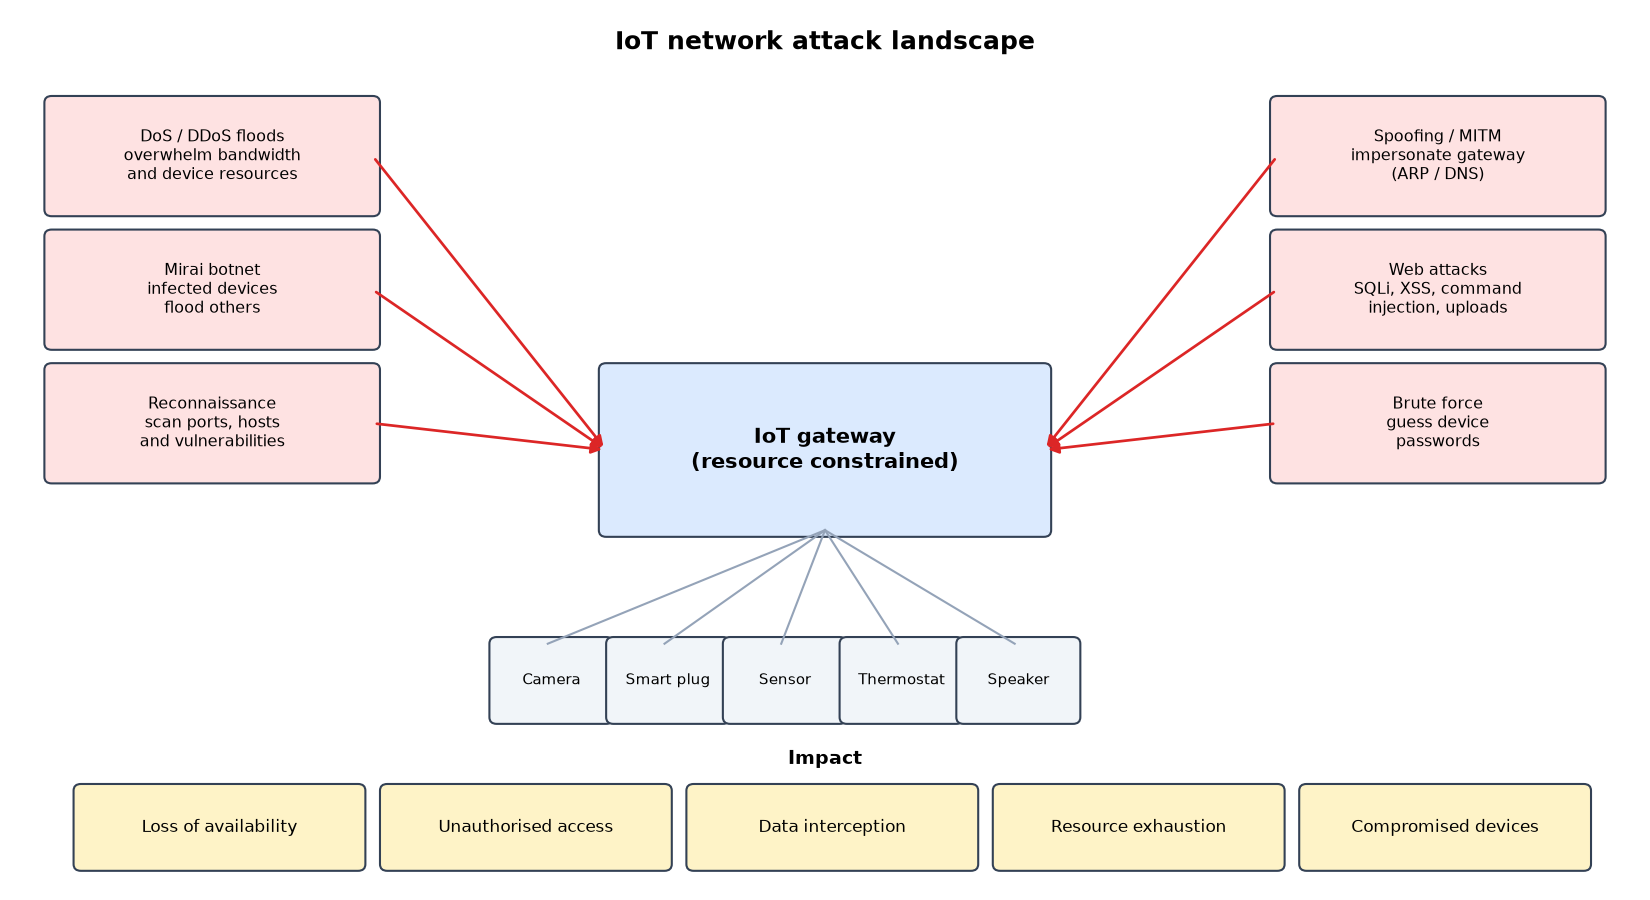
\includegraphics[width=\linewidth]{iot_attack_landscape.png}
    \caption{IoT network attack landscape and potential impact of cyberattacks.}
    \label{fig:iot_attack_landscape}
\end{figure}

To address this requirement, Intrusion Detection Systems (IDS) are used to monitor network traffic and identify suspicious or malicious activities. An IDS analyses the traffic or the features associated with the incoming traffic\cite{abdulganiyu2023systematic}, helps identify normal versus malicious behaviour, and raises an alert when suspicious activity is detected. Traditional IDS approaches may rely on predefined signatures or rules, which can limit their ability to recognise changing attack patterns\cite{khraisat2019survey}. Therefore, ML and DL-based approaches have been explored, because they can learn patterns from network traffic without relying only on predefined attack signatures\cite{rakine2025comprehensive}. ML-based IDS approaches can perform binary classification, where network traffic is classified as either normal or malicious. However, binary classification does not provide information about the specific type of attack\cite{palshikar2022distinguishes}, and different types of attacks need to be mitigated with different responses. A multiclass IDS can further classify malicious traffic into specific attack categories, providing more detailed information about the nature of the detected attack. However, although ML/DL-based multiclass IDS can provide detailed attack classification, their computational and memory requirements can make deployment challenging in resource-constrained IoT environments\cite{mallidi2025advancements}.

Due to the limited resources and memory of IoT devices, running a complex ML/DL-based model can be a problem. Therefore, lightweight and resource-efficient IDS models are required for resource-constrained IoT environments\cite{arshad2020intrusion}. For this, resource optimisation techniques can be used to reduce the resource requirements of ML/DL models, and one of these approaches is quantization\cite{gholami2022survey}. Quantization reduces the numerical precision used to represent the parameters of a model, which reduces the model size and computational requirements while maintaining detection performance. Therefore, quantizing the IDS can make the multiclass detection system more suitable for resource-constrained IoT environments\cite{misrak2025lightweight}.

But resource efficiency alone cannot address the challenge of detecting previously unseen or zero-day attacks\cite{el2024advanced}. Existing IDS and ML/DL-based models are trained using known traffic and attack patterns, and when traffic behaves differently from the patterns seen during training\cite{sabeel2021building}, classification of attacks can be difficult. Therefore, detecting abnormal behaviour is important in addition to classifying known attack types. Anomaly detection can identify traffic behaviour that differs from normal behaviour, which makes it useful for detecting potentially unseen attack patterns. One traffic characteristic that can be used for identifying unseen attacks is the packet Inter-Arrival Time (IAT), which is the interval of time between two consecutive packets\cite{sahin2025leveraging}.

\begin{figure}[htbp]
    \centering
    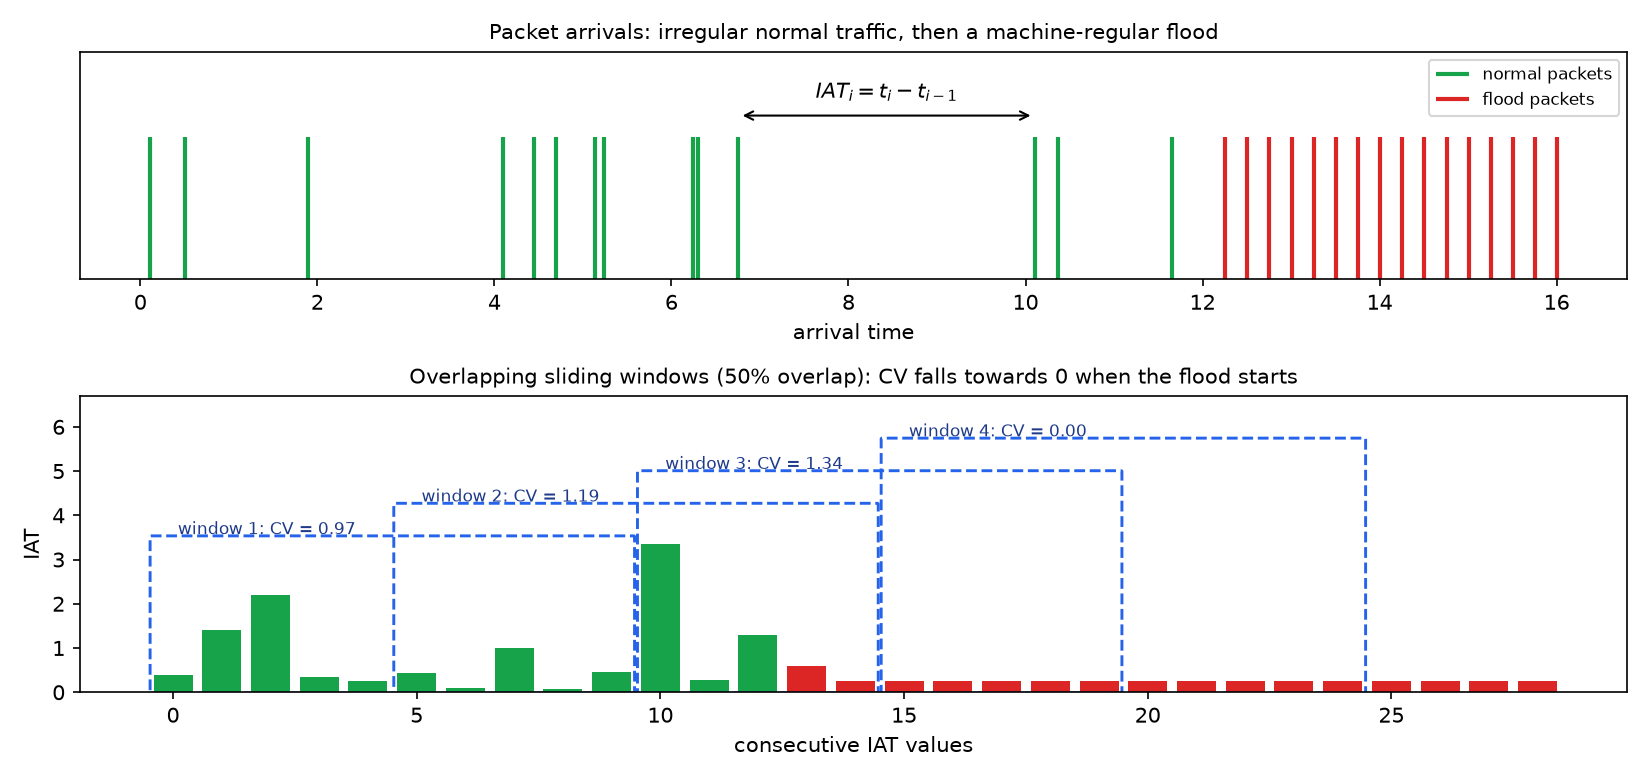
\includegraphics[width=\linewidth]{iat_diagram.png}
    \caption{Illustration of Packet Inter-Arrival Time (IAT) and sliding windows over consecutive IAT values.}
    \label{fig:iat}
\end{figure}

To analyse the variations in packet inter-arrival time, a sliding-window approach can be used to check the traffic behaviour over the incoming packets. In each window, the IAT values of the incoming consecutive packets are considered and their standard deviation is calculated to measure the variation in packet arrival time and frequency. If the behaviour of the window is found to be abnormal, the traffic is considered potentially anomalous, and this anomaly can trigger the multiclass IDS for further classification of the suspicious traffic\cite{toupas2019intrusion}. The multiclass IDS can classify the suspicious traffic into the corresponding attack category based on the traffic patterns, and based on the identified type an appropriate mitigation technique can be applied to the incoming suspicious traffic; for example, rate limiting and traffic filtering are used to mitigate DDoS attacks. After applying the specific mitigation technique, the network can be analysed again to determine whether the abnormal behaviour of the traffic has been reduced, and if the abnormal behaviour is still present, further mitigation can be initiated.

Based on the above challenges, there is a need for an IoT intrusion detection system that can address resource constraints, detect abnormal attack behaviour and also support appropriate mitigation\cite{heidari2023internet}. Therefore, this work proposes the Inter-Arrival Time based Fuzzy detection, Classification and Mitigation (IATFCM) algorithm for IoT networks and devices. IATFCM uses the packet inter-arrival time with sliding-window analysis to identify abnormal traffic behaviour. A quantized multiclass IDS is then used to classify the suspicious traffic into different categories of attack, and based on the identified type of attack an appropriate mitigation technique is applied\cite{mondal2026quantized}, followed by re-analysis of the network traffic to verify the reduction of the anomaly. The overall approach aims to provide a lightweight and resource-efficient mechanism for detecting, classifying and mitigating malicious activities in resource-constrained IoT networks.

\subsection{Contributions}
The main contributions of this work are:
\begin{enumerate}
\item \textbf{The IATFCM algorithm}, which places a label-free fuzzy gate in front of a quantized multiclass classifier and an attack-specific mitigation stage. In an end-to-end stream, 57.4\% of the windows never reached the classifier, the computation per window fell by 35.5\%, and the benign windows that received a mitigation plan fell from 32 to 3.
\item \textbf{A fuzzy detector that combines inter-arrival time statistics with a behaviour deviation learned only from benign traffic.} It raises the recall from 14.6\% (timing inputs only) to 96.2\%, detects every window of an unseen attack family, and uses a rule base refined through an ablation study.
\item \textbf{An attack-vote rule and a nearest-neighbour zero-day check for the classifier.} The vote raises the window accuracy from 86.9\% to 98.5\%, and the check recognises all unseen Mirai windows as unknown, against 58.3\% for confidence-based rejection and 0\% for the compared classifiers.
\item \textbf{An INT8 classifier with integer-only matrix arithmetic} that needs 16.2~KB, 74.6\% less than its FP32 version, with 98.5\% identical predictions.
\item \textbf{Verified attack-specific mitigation} with 10 policy families and shape-based ladders for unseen attacks, which verified 96.1\% of the mitigations across 33 attack classes; escalation raises the resolved attacks from 89.6\% to 99.4\%, and targeted filtering drops 14.6\% of the legitimate records instead of 100\%.
\item \textbf{An evaluation under one protocol} against five re-implemented existing algorithms and the published results of two more, together with an ablation study of every component.
\end{enumerate}

The rest of the paper is organised as follows. Section~\ref{sec:lit} reviews the related works and gives each of them a short name. Section~\ref{sec:iatfcm} presents the proposed IATFCM algorithm, the dataset and the three modules. Section~\ref{sec:ablation} reports the ablation study, Section~\ref{sec:results} compares IATFCM with the existing algorithms, and Section~\ref{sec:conclusion} concludes the paper.


% =====================================================================================
\section{Literature Survey}\label{sec:lit}
% =====================================================================================
This section reviews recent intrusion detection works that are closest to IATFCM in their goals: lightweight detection, use of timing behaviour, quantization, and handling of IoT traffic. Each work is given a short name, which is used for the comparison in Section~\ref{sec:results}.

Ertam and Aydogmus\cite{ertam2026privacy} proposed a privacy-preserving IDS for Wi-Fi-enabled robotic platforms, which we refer to as PP-TTF (Privacy-Preserving Temporal Traffic Features). The detector never looks at packet payloads or addresses; instead it engineers 26 descriptors from the packet inter-arrival time alone, such as the entropy and the coefficient of variation of the IAT over rolling windows of 3, 5 and 10 packets and burst counters, balances the classes with SMOTE, and compares Random Forest, SVM, MLP, gradient boosting and LSTM classifiers. On 36,098 samples of five classes recorded from a real robot, the best binary model reached an F1-score of 0.906 and the best multiclass model an accuracy of 0.782. The authors observe that IAT features describe high-rate attacks that disrupt connectivity well, but give limited separation for low-rate attacks, and the work does not consider unseen attacks or any response to a detected attack.

\c{S}olpan et al.\cite{solpan2026hybrid} split the Wi-Fi traffic of the AWID3 dataset into multivariate time-series blocks and derived two representations of every block, statistical descriptors and CNN-based features, which were classified with KNN, SVM, XGBoost and voting ensembles over 24 experimental configurations. We call this approach HFF-XGB (Hybrid Feature Fusion with XGBoost), after its strongest combination, XGBoost on the statistical descriptors, which exceeded 0.98 in both accuracy and F1-score on 14 classes. The approach computes a large set of attributes for every block, which adds latency on constrained devices, and as a supervised model it can only output the classes seen in training; mitigation is not addressed.

Nie et al.\cite{nie2025intrusion} detect compromised nodes in wireless networks through traffic anomaly analysis, an approach we denote SAE-PSVM (Stacked AutoEncoder with Particle-swarm-optimised SVM). The traffic collected from the nodes is cleaned and reconstructed, a stacked autoencoder compresses it into standardised anomaly profiles, and an SVM whose parameters are tuned by particle swarm optimisation classifies them, keeping the false detection rate below 6\%. The multi-stage pipeline is heavy in computation and memory, and it stops at flagging the compromised node without a countermeasure.

Tuman et al.\cite{tuman2025edge} designed BCT (Boosted Convolutional Trees) for edge IoT devices: a compact 1D convolutional front-end without pooling feeds an ensemble of differentiable soft decision trees that is trained end to end and boosted. On CICIoT2023, X-IIoTID and Edge-IIoTset, BCT stays within a few points of CNN and LSTM baselines while being much smaller and faster, cutting the latency by 67.7\% on average; on CICIoT2023 it reports a macro-F1 of 0.4747 with a 0.10~MB model and 0.1131~ms per sample. The authors point out that class imbalance limits its performance and that it was not deployed on physical hardware.

Misrak and Melaku\cite{misrak2025lightweight} proposed a quantized hybrid deep network, DNN-BiLSTMQ. Features are selected with redundancy-adjusted logistic mutual-information feature selection (RAL-MIFS) and reduced with a two-stage incremental PCA, quantization-aware training and post-training dynamic quantization shrink the model, and Optuna tunes the hyperparameters. The model reaches 99.73\% accuracy with 25.6~KB on CIC-IDS2017 and 93.95\% accuracy with 31.3~KB on CICIoT2023. Minority attack classes remain difficult, and the model was not evaluated on a resource-constrained device.

A lightweight dynamic-threshold detector for edge devices\cite{dynamic_ids2025}, denoted DT-3$\sigma$ here, follows only two features, packets per second and bytes per second, over a 30-second sliding window and raises an alarm when a value leaves the band of the mean plus or minus three standard deviations, with a Kolmogorov--Smirnov normality check and protocol-aware filtering. It reports 94.7--96.2\% accuracy with 5.1\% CPU usage on CICIDS2017, NSL-KDD and simulated industrial traffic, but it assumes approximately normal traffic and reacts poorly to non-stationary patterns such as periodic spikes.

Umar et al.\cite{umar2025energy} proposed DNN-KDQ, an energy-efficient deep neural network for edge intrusion detection that is compressed by knowledge distillation and quantization. Using energy-centric features of CICIDS2017 and adaptive sampling, the distilled and quantized student network reaches 99.43\% accuracy, while the model shrinks from 196.77~KB to 20.18~KB and infers in 0.07~ms per sample. The evaluation uses one older dataset, and like the other supervised works it does not consider unseen attacks or mitigation.

Table~\ref{tab:lit} summarises these works. Most of them stop at detection or classification, only one deals with attacks that are absent from training, and none applies and then verifies a response.

\begin{table}[htbp]
\tbl{Summary of the related works and their short names (\checkmark: addressed, --: not addressed).}
{\small
\begin{tabular}{llllcccc}
\toprule
Short name & Ref. & Dataset & Core technique & Multiclass & Unseen & Lightweight & Mitigation \\
\midrule
PP-TTF      & \cite{ertam2026privacy}     & Robotic Wi-Fi & 26 IAT features + ML         & \checkmark & -- & \checkmark & -- \\
HFF-XGB     & \cite{solpan2026hybrid}     & AWID3         & Block statistics + XGBoost   & \checkmark & -- & --         & -- \\
SAE-PSVM    & \cite{nie2025intrusion}     & Wireless      & Stacked AE + PSO-SVM         & --         & partial & -- & -- \\
BCT         & \cite{tuman2025edge}        & CICIoT2023 +2 & Conv. + soft boosted trees   & \checkmark & -- & \checkmark & -- \\
DNN-BiLSTMQ & \cite{misrak2025lightweight}& CICIoT2023 +1 & DNN-BiLSTM + QAT/PTDQ        & \checkmark & -- & \checkmark & -- \\
DT-3$\sigma$& \cite{dynamic_ids2025}      & CICIDS2017 +2 & 3$\sigma$ rate thresholds    & --         & \checkmark & \checkmark & -- \\
DNN-KDQ     & \cite{umar2025energy}       & CICIDS2017    & Distillation + quantization  & \checkmark & -- & \checkmark & -- \\
\textbf{IATFCM} & --                      & CICIoT2023    & IAT fuzzy + INT8 + policies  & \checkmark & \checkmark & \checkmark & \checkmark \\
\bottomrule
\end{tabular}}
\label{tab:lit}
\end{table}

\subsection{Motivation}
The survey shows three gaps. First, detectors that use only timing statistics (PP-TTF, DT-3$\sigma$) are light and privacy-preserving, but they miss attacks that do not change the timing of the traffic, and a simple threshold reacts poorly to the heavy-tailed rates of IoT traffic. Second, supervised classifiers (HFF-XGB, BCT, DNN-BiLSTMQ, DNN-KDQ) name the attack, but they always answer with a known class, so an unseen attack is silently mislabelled, and most of them run on every record, which is costly on a gateway. Third, none of the works applies a response and checks whether it worked, although the purpose of naming the attack is to choose the right response. IATFCM addresses these gaps by placing a label-free fuzzy gate in front of a quantized classifier with an open-set check, and by closing the loop with attack-specific mitigation that is verified by the same gate.


% =====================================================================================
\section{Inter-Arrival Time Based Fuzzy Detection, Classification and Mitigation (IATFCM) Algorithm}\label{sec:iatfcm}
% =====================================================================================
IATFCM is a three-stage algorithm that decides, for every window of IoT traffic, whether the window is anomalous, which attack it contains, and how to respond to it. The design follows one principle: the cheapest test runs on every window, and the more expensive steps run only when the cheaper one asks for them. The first stage (Module 1) is a Mamdani fuzzy inference system\cite{mamdani1975experiment} that turns the inter-arrival time statistics of a window of $W = 20$ flow records, together with a behaviour deviation learned only from normal traffic, into a continuous attack risk. It needs no attack labels, so it is the part of IATFCM that can notice an attack it has never seen. When the risk stays in the normal zone, the window is forwarded and nothing else is computed. When it does not, the second stage (Module 2) classifies every record of the window and decides the window's attack class by a vote, using either a Random Forest\cite{breiman2001random} or an 8-bit integer neural network for constrained devices\cite{jacob2018quantization}. Because a supervised classifier can only answer with a class it knows, Module 2 also measures how far the window lies from all known training traffic, and labels it as a possible zero-day attack when it is too far away.

The third stage (Module 3) turns the decision into an action. A known attack class is looked up in a policy table, which maps each class to a family of attacks that are stopped in the same way and gives an escalation ladder that starts with the least disruptive action. An unknown attack has no class to look up, so its ladder is chosen from the shape of its traffic, using the same timing features that Module 1 has already measured. Filtering actions on confidently classified attacks may run automatically, while blocking or isolating traffic always waits for an analyst. After every action the window is scored again by Module 1, and IATFCM escalates to the next action until the risk is back in the normal zone. In this way the detector that raised the alarm is also the judge of whether the response worked.

Three properties follow from this design. The classifier and the mitigation logic are idle for most normal traffic, which saves computation on the gateway. Unseen attacks are caught twice, by the label-free risk of Module 1 and by the distance check of Module 2, and they still receive a containment action. Finally, every decision can be explained: the fuzzy rules that fired, the class probabilities and votes, the policy or traffic shape that chose the action, and the risk before and after it. The overall workflow is shown in Fig.~\ref{fig:workflow}, the complete procedure is given in Algorithm~\ref{alg:iatfcm}, and the symbols are listed in Table~\ref{tab:symbols}.

\begin{table}[htbp]
\tbl{Symbols used in IATFCM.}
{\small
\begin{tabular}{ll}
\toprule
Symbol & Description \\
\midrule
$W$, $S$ & Window size (20 records) and step between windows \\
$\mathrm{IAT}_i$, $\mathrm{Rate}_i$ & Inter-arrival time and packet rate of record $i$ \\
$\mu_t$, $\sigma_t$, $CV_t$ & Mean, standard deviation and coefficient of variation of the IAT in window $t$ \\
$\tilde{R}_t$, $D_t$, $B_t$ & Median packet rate, IAT deviation and behaviour deviation of window $t$ \\
$\mu_N$, $\theta_B$ & Mean normal IAT and behaviour threshold, from benign training traffic \\
$A_t$, $A'_t$ & Attack risk of window $t$ before and after a mitigation action \\
$\hat{c}_t$, $p_t$ & Window class decided by the vote and its confidence \\
$Z_t$, $\theta_Z$ & Zero-day score of window $t$ and its calibration threshold \\
$\Pi$, $\mathcal{L}_t$ & Policy table and escalation ladder selected for window $t$ \\
$e_s$, $S_t$ & Assumed efficacy of action $s$ and share of targeted traffic removed \\
\bottomrule
\end{tabular}}
\label{tab:symbols}
\end{table}

\unhead{Dataset}
IATFCM is designed and evaluated with CICIoT2023\cite{neto2023ciciot2023}, a large IoT intrusion dataset released by the Canadian Institute for Cybersecurity. The traffic was captured in a testbed of 105 real IoT devices, such as cameras, smart plugs, sensors and smart speakers, while malicious IoT devices executed 33 attacks against the other devices. The attacks belong to seven families: DDoS (12 classes), DoS (4), Mirai botnet (3), reconnaissance (5), spoofing (2), web-based attacks (6) and brute force (1), and benign traffic forms the 34th class. The captured packets were converted by the dataset's feature extractor into flow-level records, and each record has 46 numeric features and a label. We use the public CSV release, which contains a training file of 1.6~GB and a separate test file of 348~MB. Three properties of this release shape our design. The classes are strongly imbalanced, with DDoS floods dominating and some web classes having fewer than 150 test records. The files contain no packet timestamps, so the extractor's IAT feature is the timing signal. Finally, the rows are shuffled, so windows are assembled from records of the class under evaluation together with benign background records.

Because the training file is too large for a constrained setting, it is read in chunks and capped at 6,000 records per class, which gives 153,135 training records; the test file gives 37,187 test records with a cap of 1,500 per class (Table~\ref{tab:dataset}). The test records are never used for training or calibration. The whole Mirai family is held out of every supervised model, threshold and policy, so that it can serve as a realistic unseen attack. Table~\ref{tab:features} lists the 46 features in four groups and shows which part of IATFCM uses them. Module 1 computes its timing statistics from only two columns, \texttt{IAT} and \texttt{Rate}, while its behaviour deviation, Module 2 and the shape test of Module 3 use the full feature vector. The \texttt{label} column is used only to train Module 2 and to evaluate the results.

\begin{table}[htbp]
\tbl{CICIoT2023 records used in this work, by attack family.}
{\small
\begin{tabular}{lccc}
\toprule
Family & Classes & Training records & Test records \\
\midrule
Benign       & 1  & 6,000  & 1,500 \\
DDoS         & 12 & 66,128 & 16,331 \\
DoS          & 4  & 24,000 & 5,771 \\
Reconnaissance & 5 & 22,645 & 5,140 \\
Spoofing     & 2  & 12,000 & 3,000 \\
Web-based    & 6  & 2,821  & 626 \\
Brute force  & 1  & 1,541  & 319 \\
Mirai (held out as unseen) & 3 & 18,000 (not used) & 4,500 \\
\midrule
Total        & 34 & 153,135 & 37,187 \\
\bottomrule
\end{tabular}}
\label{tab:dataset}
\end{table}

\begin{table}[htbp]
\tbl{The 46 CICIoT2023 features and their use in IATFCM.}
{\small
\begin{tabular}{p{2.6cm}p{7.6cm}p{2.6cm}}
\toprule
Group & Features & Used by \\
\midrule
Timing and rate (6) & \texttt{IAT}, \texttt{Rate}, \texttt{Srate}, \texttt{Drate}, \texttt{flow\_duration}, \texttt{Duration} & M1 (\texttt{IAT}, \texttt{Rate}), $B_t$, M2, M3 \\
Header and flags (13) & \texttt{Header\_Length}; FIN, SYN, RST, PSH, ACK, ECE and CWR flag numbers; ACK, SYN, FIN, URG and RST counts & $B_t$, M2 \\
Protocol indicators (15) & \texttt{Protocol Type}, HTTP, HTTPS, DNS, Telnet, SMTP, SSH, IRC, TCP, UDP, DHCP, ARP, ICMP, IPv, LLC & $B_t$, M2 \\
Size statistics (12) & \texttt{Tot sum}, \texttt{Min}, \texttt{Max}, \texttt{AVG}, \texttt{Std}, \texttt{Tot size}, \texttt{Number}, \texttt{Magnitue}, \texttt{Radius}, \texttt{Covariance}, \texttt{Variance}, \texttt{Weight} & $B_t$, M2 \\
Label & \texttt{label} (34 classes) & training and evaluation only \\
\bottomrule
\end{tabular}}
\label{tab:features}
\end{table}

\unhead{Working of the modules in brief}
IATFCM processes the traffic as a stream of overlapping windows of 20 flow records. For every window, \textbf{Module 1} computes four values: the coefficient of variation of the inter-arrival times, which collapses towards zero for machine-generated floods and grows for irregular probing; the median packet rate; the deviation of the mean IAT from normal traffic; and a behaviour deviation, which measures how far the window's records are from their nearest benign training records. The Mamdani system fuzzifies the four values into Low, Medium and High degrees, applies 15 rules and defuzzifies the result into an attack risk between 0 and 1. A risk below 0.35 forwards the window, and anything higher sends it to Module 2. \textbf{Module 2} classifies each of the 20 records and takes the majority class among the records that look like an attack, so that a few benign background records do not hide the attack. It then computes the zero-day score of the attack records. If the score is above its threshold, the window is reported as an unknown attack; if only benign records are found, Module 2 overrules Module 1's alarm. \textbf{Module 3} routes a known class to its policy family and an unknown window to a ladder chosen by its traffic shape, decides whether the first action may run automatically, applies the action to the records that Module 2 marked as attacks, and re-scores the window with Module 1. The ladder is escalated until the risk falls below 0.35, or the incident is passed to the security team when the ladder is exhausted.

\begin{figure}[htbp]
\centering
\resizebox{\textwidth}{!}{%
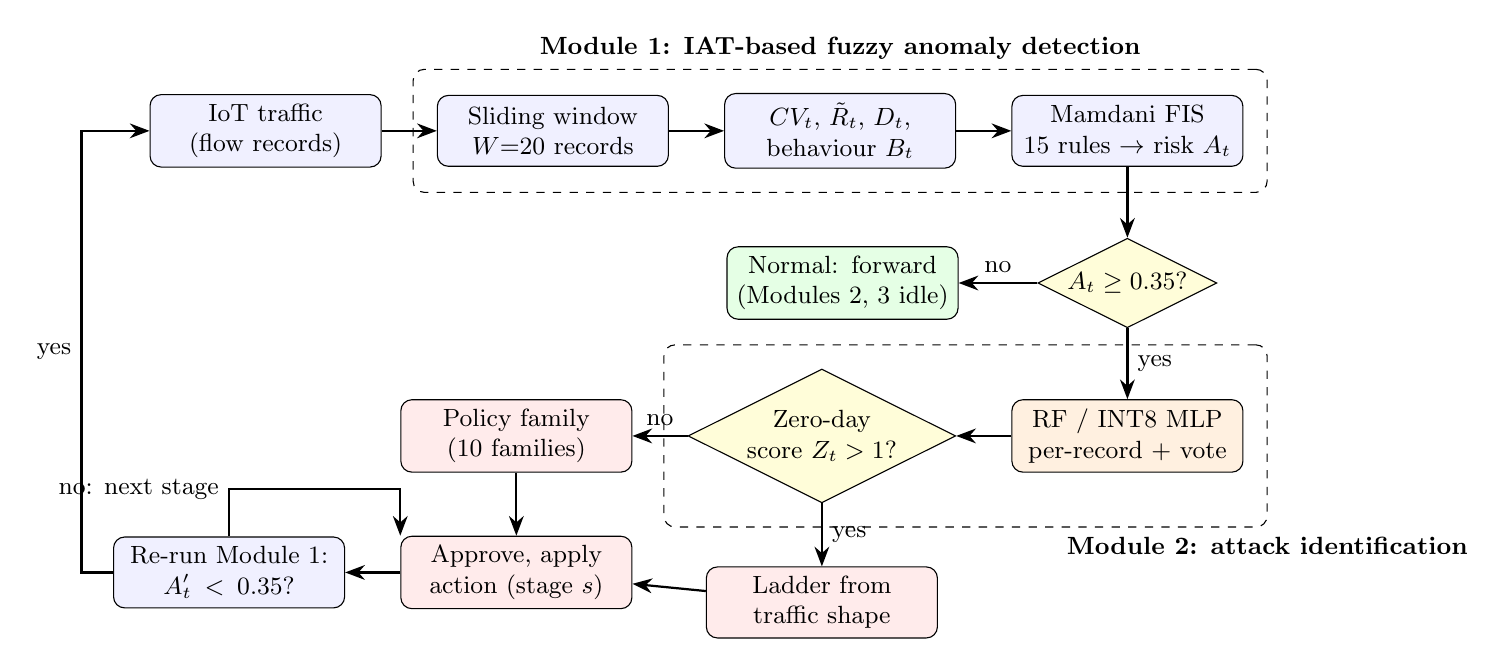
\begin{tikzpicture}[
  node distance=5mm and 7mm,
  box/.style={draw, rounded corners, align=center, minimum height=9mm, text width=27mm, font=\small, fill=blue!6},
  m2/.style={box, fill=orange!12},
  m3/.style={box, fill=red!8},
  ok/.style={box, fill=green!10},
  dec/.style={draw, diamond, aspect=2, align=center, font=\small, inner sep=1pt, fill=yellow!15},
  arr/.style={-{Stealth[length=2.5mm]}, thick}]
\node[box] (in) {IoT traffic\\(flow records)};
\node[box, right=of in] (win) {Sliding window\\$W{=}20$ records};
\node[box, right=of win] (feat) {$CV_t$, $\tilde{R}_t$, $D_t$,\\behaviour $B_t$};
\node[box, right=of feat] (fis) {Mamdani FIS\\15 rules $\rightarrow$ risk $A_t$};
\node[dec, below=9mm of fis] (gate) {$A_t \ge 0.35$?};
\node[ok, left=10mm of gate] (pass) {Normal: forward\\(Modules 2, 3 idle)};
\node[m2, below=9mm of gate] (clf) {RF / INT8 MLP\\per-record + vote};
\node[dec, left=of clf] (zd) {Zero-day\\score $Z_t>1$?};
\node[m3, below=8mm of zd] (shape) {Ladder from\\traffic shape};
\node[m3, left=of zd] (pol) {Policy family\\(10 families)};
\node[m3, below=8mm of pol] (act) {Approve, apply\\action (stage $s$)};
\node[box, left=of act] (ver) {Re-run Module 1:\\$A'_t<0.35$?};
\begin{scope}[on background layer]
\node[draw, dashed, rounded corners, fit=(win)(feat)(fis), inner sep=3mm, label={[font=\small\bfseries]above:Module 1: IAT-based fuzzy anomaly detection}] {};
\node[draw, dashed, rounded corners, fit=(clf)(zd), inner sep=3mm, label={[font=\small\bfseries]below right:Module 2: attack identification}] {};
\end{scope}
\draw[arr] (in) -- (win);
\draw[arr] (win) -- (feat);
\draw[arr] (feat) -- (fis);
\draw[arr] (fis) -- (gate);
\draw[arr] (gate) -- node[above,font=\small]{no} (pass);
\draw[arr] (gate) -- node[right,font=\small]{yes} (clf);
\draw[arr] (clf) -- (zd);
\draw[arr] (zd) -- node[above,font=\small]{no} (pol);
\draw[arr] (zd) -- node[right,font=\small]{yes} (shape);
\draw[arr] (pol) -- (act);
\draw[arr] (shape) -- (act);
\draw[arr] (act) -- (ver);
\draw[arr] (ver.north) -- ++(0,6mm) node[left,font=\small]{no: next stage} -| (act.north west);
\draw[arr] (ver.west) -- ++(-4mm,0) |- node[near start,left,font=\small]{yes} (in.west);
\end{tikzpicture}}
\caption{Workflow of the IATFCM algorithm. Module 1 checks every window, only suspicious or attack windows reach Module 2, and Module 3 applies the policy-based or shape-based action and verifies it with Module 1.}
\label{fig:workflow}
\end{figure}

\begin{algorithm}[htbp]
\caption{The IATFCM algorithm}
\label{alg:iatfcm}
\small
\begin{algorithmic}[1]
\Require stream of flow records; $W$ = window size; $\mu_N$, $\theta_B$ = normal baseline; FIS = fuzzy rule base; $f$ = Random Forest or INT8 classifier; $\theta_Z$ = zero-day threshold; $\Pi$ = policy table
\Ensure decision for each window (normal / attack class / zero-day) and a verified mitigation
\Step{1} set $W = 20$, $S = 10$; load $\mu_N$, $\theta_B$, FIS, $f$, $\theta_Z$ and $\Pi$
\While{flow records arrive}
  \Step{2} \Comment{Module 1: anomaly detection}
  \State form window $t$ of the last $W$ records
  \State compute $\mu_t$, $\sigma_t$, $CV_t = \sigma_t/\mu_t$, $\tilde{R}_t$, $D_t = |\mu_t-\mu_N|/\mu_N$ and $B_t$
  \State $A_t \gets$ FIS$(CV_t, \tilde{R}_t, D_t, B_t)$ \Comment{fuzzify, 15 rules, centroid}
  \If{$A_t < 0.35$}
    \State forward the window; Modules 2 and 3 stay idle; \textbf{continue}
  \EndIf
  \Step{3} \Comment{Module 2: attack identification}
  \State classify every record with $f$; $\hat{c}_t \gets$ majority class among the attack records
  \State $Z_t \gets$ median nearest-known distance of the attack records $/\ \theta_Z$
  \If{$\hat{c}_t = $ Benign \textbf{and} $Z_t \le 1$}
    \State mark the alarm as false; \textbf{continue}
  \EndIf
  \Step{4} \Comment{Module 3: mitigation and verification}
  \If{$Z_t > 1$}
    \State $\mathcal{L}_t \gets$ ladder of the traffic shape of the attack records (Table~\ref{tab:shape})
  \Else
    \State $\mathcal{L}_t \gets \Pi[\hat{c}_t]$ \Comment{policy family of the class}
  \EndIf
  \For{$s = 1$ \textbf{to} $|\mathcal{L}_t|$}
    \If{action $\mathcal{L}_t[s]$ blocks traffic \textbf{or} $p_t <$ policy threshold}
      \State request analyst approval
    \EndIf
    \State apply $\mathcal{L}_t[s]$ to the records marked as attack
    \State $A'_t \gets$ FIS of the window after the action
    \If{$A'_t < 0.35$}
      \State mark the attack as resolved; \textbf{break}
    \EndIf
  \EndFor
  \If{the attack is not resolved}
    \State escalate the incident to the security team
  \EndIf
\EndWhile
\end{algorithmic}
\end{algorithm}


% -------------------------------------------------------------------------------------
\subsection{Module 1: IAT-based fuzzy anomaly detection}\label{sec:m1}
% -------------------------------------------------------------------------------------
Module 1 decides whether a window is anomalous. It is the only module that runs on every window, so it uses a few statistics that are cheap to compute and a rule base that can be read and checked.

\textbf{Windows and labels.} The records are grouped into windows of $W = 20$ consecutive records, and in a live deployment consecutive windows overlap by 50\% (step $S = 10$). For evaluation, the label of a window follows the share of attack records in it:
\begin{equation}
  a_t = \frac{1}{W}\sum_{i=1}^{W} \mathbf{1}\!\left(y_i \neq \text{Benign}\right),
  \qquad
  y_t = \begin{cases} 1, & a_t \ge 0.5\\ 0, & \text{otherwise} \end{cases}
\end{equation}
where $y_i$ is the label of record $i$, $a_t$ is the share of attack records in window $t$ and $y_t$ is the window label.

\textbf{Timing features.} From the IAT values of the window, the mean, the standard deviation and the coefficient of variation are calculated:
\begin{equation}
  \mu_t = \frac{1}{W}\sum_{i=1}^{W}\mathrm{IAT}_i,\qquad
  \sigma_t = \sqrt{\frac{1}{W}\sum_{i=1}^{W}\left(\mathrm{IAT}_i-\mu_t\right)^2},\qquad
  CV_t = \frac{\sigma_t}{\mu_t + \epsilon}
\end{equation}
with $\epsilon = 10^{-12}$. Normal IoT traffic has natural jitter, and the median CV of benign training windows is 1.00. Flooding tools send packets at an almost constant interval, so their CV collapses: the median window CV is 0.001 for DDoS and below 0.001 for DoS in our data. Irregular probes raise the CV instead. The traffic volume is described by the median packet rate $\tilde{R}_t = \operatorname{Median}(\mathrm{Rate}_1,\ldots,\mathrm{Rate}_W)$, because the rate feature is heavy-tailed and a single benign record with an extreme rate would otherwise lift the mean of the whole window. The IAT deviation compares the mean IAT with the normal mean $\mu_N$:
\begin{equation}
  D_t = \frac{\left|\mu_t-\mu_{N}\right|}{\mu_{N}}
\end{equation}

\textbf{Behaviour deviation.} Timing alone misses attacks that leave the timing of the traffic unchanged, such as reconnaissance, spoofing and web attacks, and a few benign records in a flood window are enough to break its regular timing. A fourth input therefore measures how unusual the records themselves are. The 46 features of each record are compressed with $x \mapsto \operatorname{sign}(x)\log(1+|x|)$ and standardised with the statistics of benign training records, $d_i$ is the mean Euclidean distance of record $i$ to its $k = 5$ nearest benign training records, and
\begin{equation}
  B_t = \frac{\operatorname{Median}\left(d_1, \ldots, d_W\right)}{\theta_B}
\end{equation}
where $\theta_B$ is the 99th percentile of the same statistic over 1,000 windows of held-out benign training records. $B_t > 1$ therefore means that the window is more unusual than 99\% of normal windows. Only normal traffic is used to build $B_t$, so Module 1 stays an unsupervised detector.

\textbf{Normal baseline.} The baseline is built from benign training traffic only and stores $\mu_N$, the median $M = \operatorname{Median}(CV)$ and the percentiles of normal window CV values, the median normal rate, and the benign reference records and threshold $\theta_B$ of the behaviour deviation. The median $M = 1.00$ is the centre of the Medium CV membership function.

\textbf{Mamdani inference.} Each input has three linguistic terms, Low, Medium and High, defined by the triangular (\texttt{trimf}) and trapezoidal (\texttt{trapmf}) membership functions of Table~\ref{tab:mf} and Fig.~\ref{fig:mf}. The 15 rules of Table~\ref{tab:rules} combine them. Rules 1--3 describe normal traffic and require normal behaviour; rules 4--12 detect timing and volume anomalies, for example rule 12 for constant-rate floods; rule 13 describes a slow, irregular probe and, as found in the ablation study (Section~\ref{sec:ablation}), requires the records to look at least somewhat unusual; rules 14 and 15 raise the risk when the records are unlike normal traffic. The strength of a rule is the minimum of its antecedent degrees, every rule clips its output set at that strength, the clipped sets are merged with the maximum operator, and the centroid gives the risk:
\begin{equation}
  A_t = \frac{\int z\,\mu_{\mathrm{agg}}(z)\,dz}{\int \mu_{\mathrm{agg}}(z)\,dz}
\end{equation}
where $z$ is the risk value and $\mu_{\mathrm{agg}}$ the merged output set. If no rule fires, the undecided value $A_t = 0.5$ is used.

\begin{table}[htbp]
\tbl{Membership functions of the fuzzy inputs and output of Module 1.}
{\small
\begin{tabular}{llll}
\toprule
Variable & Low & Medium & High \\
\midrule
$CV_t$ $[0,6]$             & trimf(0, 0, 0.65)   & trimf(0.50, $M$, 1.55)   & trapmf(1.40, 1.80, 6, 6) \\
$\tilde{R}_t$ $[0,50000]$  & trimf(0, 0, 350)    & trimf(200, 600, 1500)    & trapmf(1000, 2500, 50000, 50000) \\
$D_t$ $[0,5]$              & trimf(0, 0, 0.18)   & trimf(0.12, 0.35, 0.65)  & trapmf(0.50, 0.90, 5, 5) \\
$B_t$ $[0,10]$             & trimf(0, 0, 1.15)   & trimf(1.0, 1.3, 1.7)     & trapmf(1.4, 1.9, 10, 10) \\
$A_t$ $[0,1]$              & trimf(0, 0, 0.35)   & trimf(0.25, 0.50, 0.75)  & trapmf(0.60, 0.85, 1, 1) \\
\bottomrule
\end{tabular}}
\label{tab:mf}
\end{table}

\begin{figure}[htbp]
\centering
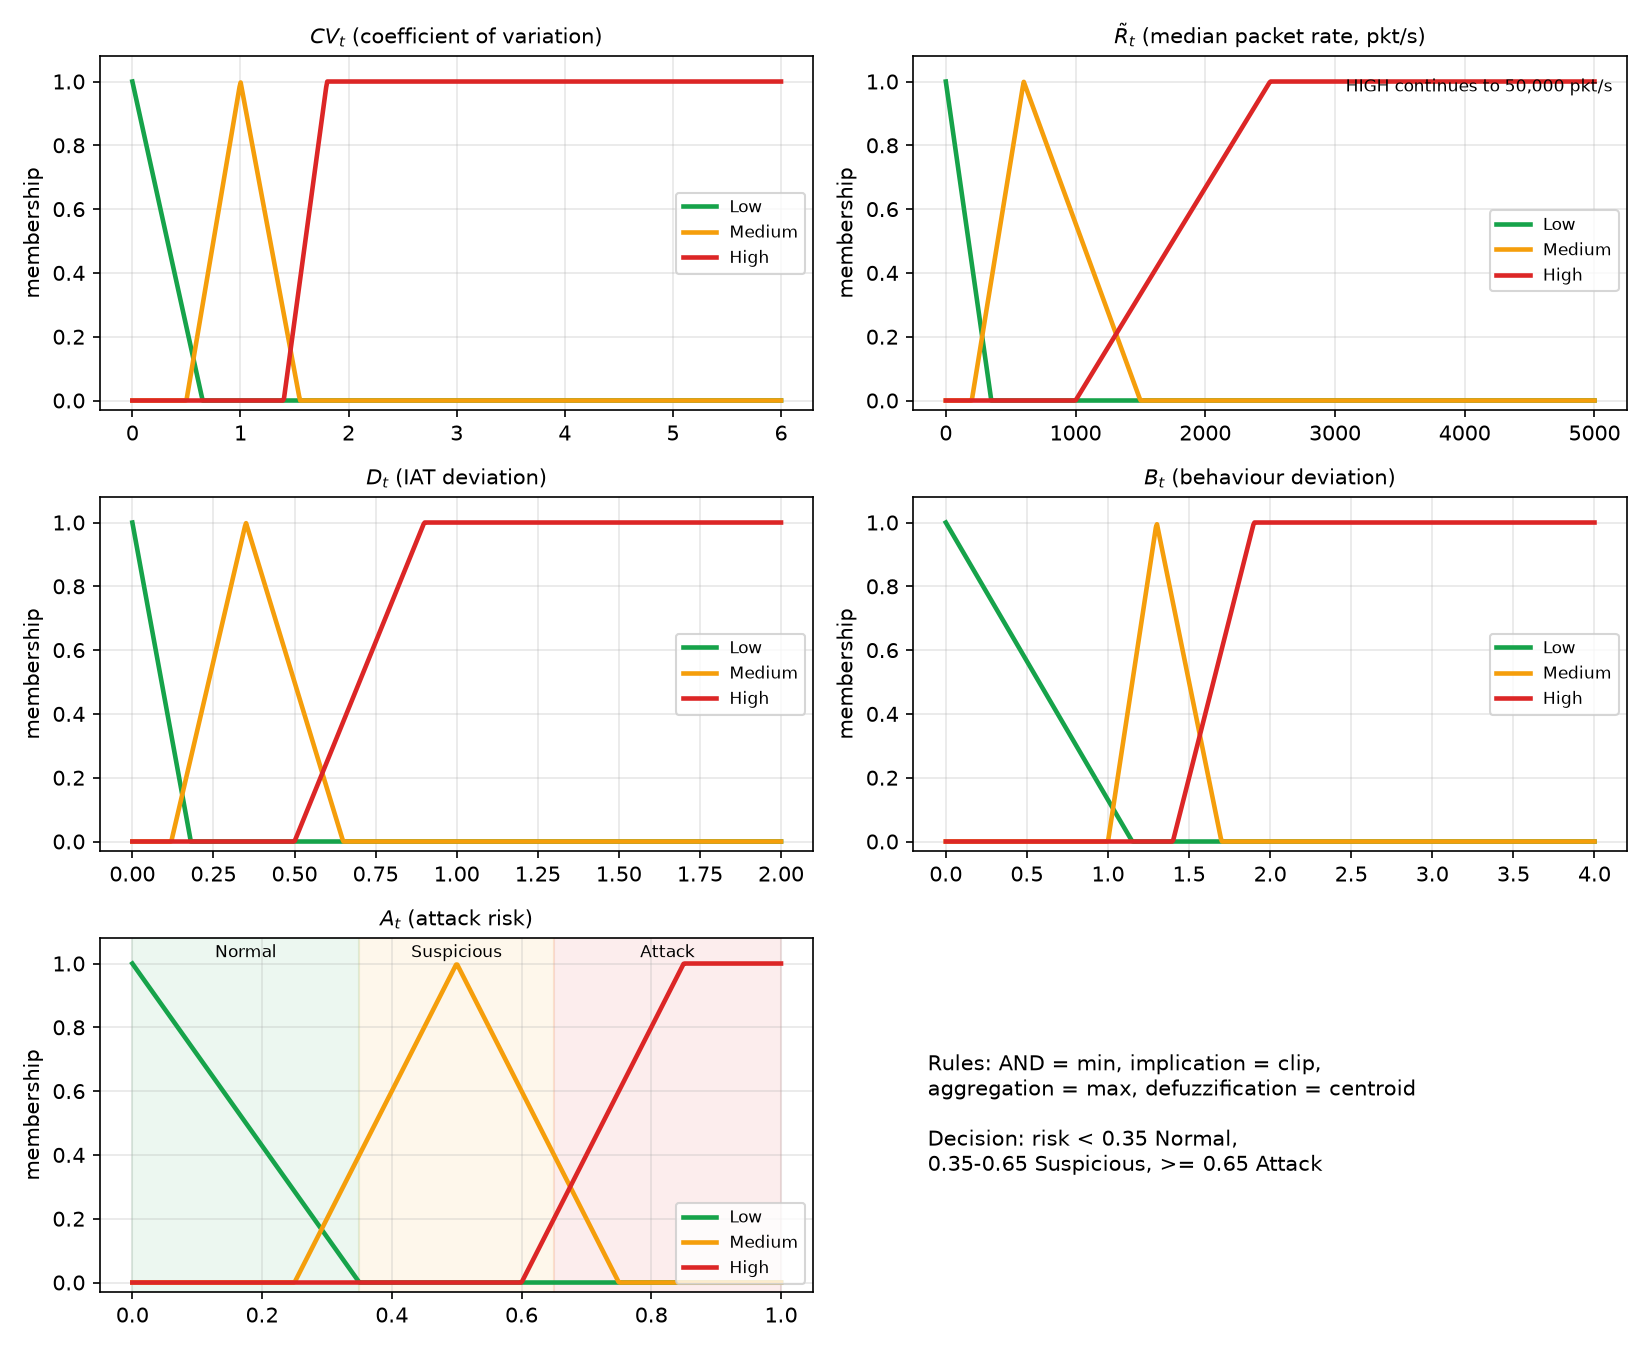
\includegraphics[width=0.95\textwidth]{fig_membership_functions.png}
\caption{Membership functions of the fuzzy inputs $CV_t$, $\tilde{R}_t$, $D_t$, $B_t$ and the output attack risk $A_t$ with the Normal, Suspicious and Attack zones.}
\label{fig:mf}
\end{figure}

\begin{table}[htbp]
\tbl{Fuzzy rule base of Module 1.}
{\small
\begin{tabular}{cll}
\toprule
\# & IF & THEN risk \\
\midrule
1  & $CV_t$ Medium $\wedge$ $\tilde{R}_t$ Low $\wedge$ $D_t$ Low $\wedge$ $B_t$ Low & Low \\
2  & $CV_t$ Low $\wedge$ $\tilde{R}_t$ Low $\wedge$ $D_t$ Low $\wedge$ $B_t$ Low & Low \\
3  & $CV_t$ Medium $\wedge$ $\tilde{R}_t$ Low $\wedge$ $D_t$ Medium $\wedge$ $B_t$ Low & Low \\
4  & $CV_t$ High $\wedge$ $\tilde{R}_t$ High & High \\
5  & $CV_t$ High $\wedge$ $D_t$ High & High \\
6  & $\tilde{R}_t$ High $\wedge$ $D_t$ High & High \\
7  & $CV_t$ Medium $\wedge$ $\tilde{R}_t$ High & High \\
8  & $CV_t$ High $\wedge$ $\tilde{R}_t$ Medium & High \\
9  & $CV_t$ Medium $\wedge$ $\tilde{R}_t$ Medium $\wedge$ $D_t$ Medium & Medium \\
10 & $\tilde{R}_t$ High & High \\
11 & $D_t$ High & High \\
12 & $CV_t$ Low $\wedge$ $\tilde{R}_t$ High & High \\
13 & $CV_t$ High $\wedge$ $\tilde{R}_t$ Low $\wedge$ $B_t$ Medium & Medium \\
14 & $B_t$ High & High \\
15 & $B_t$ Medium & Medium \\
\bottomrule
\end{tabular}}
\label{tab:rules}
\end{table}

\textbf{Decision.} The risk is mapped to three zones,
\begin{equation}
  \text{Decision}_t = \begin{cases}
    \text{Normal}, & A_t < 0.35\\
    \text{Suspicious}, & 0.35 \le A_t < 0.65\\
    \text{Attack}, & A_t \ge 0.65
  \end{cases}
\end{equation}
A normal window is forwarded and Modules 2 and 3 stay idle. A suspicious or attack window ($\hat{y}_t = 1$) is passed to Module 2.


% -------------------------------------------------------------------------------------
\subsection{Module 2: quantized multiclass attack identification}\label{sec:m2}
% -------------------------------------------------------------------------------------
Module 2 names the attack in a flagged window, or recognises that it is not a known attack. It runs only on the windows that Module 1 forwards.

\textbf{Features and training data.} Module 2 uses all 46 features of Table~\ref{tab:features}; labels are never used as input. It is trained on the 31 known classes (benign traffic and 30 attacks), with 15\% of the known training records held out for calibration. The three Mirai classes are never seen during training or calibration.

\textbf{Random Forest with attack voting.} The main classifier is a Random Forest\cite{breiman2001random} with 60 trees, a maximum depth of 20, at least 3 samples per leaf and class weights balanced per bootstrap sample. Each of the 20 records of a window is classified, and the window class is taken from the records predicted as attacks:
\begin{equation}
  \hat{c}_t = \begin{cases}
    \arg\max_{c \neq \text{Benign}} \; n_t(c), & \sum_{c \neq \text{Benign}} n_t(c) \ge 0.3\,W\\
    \text{Benign}, & \text{otherwise}
  \end{cases}
\end{equation}
where $n_t(c)$ is the number of records of window $t$ predicted as class $c$. The confidence $p_t$ is the mean predicted probability of $\hat{c}_t$ over the voting records. This rule keeps a minority of benign background records from outvoting the attack.

\textbf{INT8 edge model.} For devices that cannot hold the forest, Module 2 also provides a multilayer perceptron with the structure 46--128--64--31 (ReLU), trained with Adam (learning rate $2\times10^{-3}$, batch size 512, early stopping on 10\% of the training data). Its inputs are log-compressed and quantized to 8-bit integers with a per-feature affine quantizer fitted on the training range:
\begin{equation}
  s = \frac{r_{\max}-r_{\min}}{255}, \qquad
  z = \operatorname{round}\!\left(-128 - \frac{r_{\min}}{s}\right), \qquad
  q = \operatorname{clip}\!\left(\operatorname{round}\!\left(\tfrac{r}{s}\right) + z,\,-128,\,127\right)
\end{equation}
where $s$ is the scale, $z$ the zero point and $q$ the 8-bit value, with $r \approx s(q - z)$. After training, the input standardisation is folded into the first layer, the weights of every layer are quantized symmetrically to 8 bits ($w_q = \operatorname{round}(w/s_w)$ with $s_w = \max|w|/127$), and the activations are quantized with scales calibrated on 5,000 training records. Matrix products run as 8-bit $\times$ 8-bit $\rightarrow$ 32-bit integer accumulations\cite{jacob2018quantization}, as they would on a microcontroller.

\textbf{Zero-day check.} A closed-set classifier always answers with a known class. Rejecting low-confidence answers by their maximum softmax probability\cite{hendrycks2017baseline} is a common remedy, but unseen floods are often classified with high confidence (Section~\ref{sec:ablation}). IATFCM therefore measures distance instead. A random subset of 60,000 known training records is log-compressed, standardised and indexed, and the zero-day score of a window is
\begin{equation}
  Z_t = \frac{\operatorname{Median}_{i \in \mathcal{A}_t}\; \min_{j} \left\lVert \mathbf{x}_i - \mathbf{x}_j^{\text{train}} \right\rVert}{\theta_Z}
\end{equation}
where $\mathcal{A}_t$ is the set of records predicted as attacks and $\theta_Z$ is the 97.5th percentile of the same statistic on validation windows. The decision of Module 2 is $\hat{Y}_t = \hat{c}_t$ if $Z_t \le 1$ and $\hat{Y}_t = $ Unknown (zero-day) otherwise. Module 2 passes $\hat{Y}_t$, $p_t$, the zero-day flag and the mask of records predicted as attacks to Module 3.


% -------------------------------------------------------------------------------------
\subsection{Module 3: attack-specific mitigation and verification}\label{sec:m3}
% -------------------------------------------------------------------------------------
Module 3 decides how to respond, applies the response and checks whether it worked.

\textbf{Policies for known attacks.} The policies are kept in an external JSON file, so classes can be added without changing the code. The 31 known classes are mapped to 10 policy families, grouped by how an attack is stopped rather than by its name (Table~\ref{tab:playbooks}). For example, SYN, PSH-ACK and RST-FIN floods share the TCP state exhaustion policy because all of them are stopped by stateful filtering and SYN cookies, while UDP and ICMP floods share the volumetric flood policy. Every policy has a confidence threshold, an escalation ladder that starts with the least disruptive action, long-term recommendations and a tip for each class, for example a shorter header timeout for SlowLoris. Floods are rate-limited rather than isolated, because they mostly come from spoofed sources and isolating a local device would not stop them; scanners are blocked because they already send at a low rate; web attacks get a WAF rule so that legitimate users are not cut off. The Mirai classes are deliberately not mapped to the botnet policy, so that the unseen-attack experiment stays valid.

\begin{table}[htbp]
\tbl{Policy families and escalation ladders of Module 3 (assumed efficacy of each action in brackets).}
{\small
\begin{tabular}{lll}
\toprule
Policy family (classes) & Escalation ladder & Auto threshold \\
\midrule
Volumetric flood (UDP, ICMP, TCP, SynonymousIP floods) & rate limit (0.75) $\rightarrow$ block (0.98) $\rightarrow$ blackhole (0.97) & 0.60 \\
TCP state exhaustion (SYN, PSH-ACK, RST-FIN floods) & SYN cookies (0.80) $\rightarrow$ rate limit $\rightarrow$ block & 0.60 \\
Fragmentation (ICMP, UDP, ACK fragmentation) & drop fragments (0.80) $\rightarrow$ rate limit $\rightarrow$ block & 0.60 \\
Slow application (SlowLoris, HTTP floods) & limit connections (0.80) $\rightarrow$ block & 0.60 \\
Reconnaissance (scans, sweeps, vulnerability scan) & block scanner (0.97) $\rightarrow$ isolate segment (0.97) & 0.60 \\
Spoofing / MITM (ARP, DNS spoofing) & ARP/DNS integrity (0.95) $\rightarrow$ isolate segment & 0.65 \\
Web application (SQLi, XSS, command injection, ...) & WAF rule (0.85) $\rightarrow$ block & 0.70 \\
Credential (dictionary brute force) & throttle logins (0.85) $\rightarrow$ block & 0.70 \\
Malware / backdoor & quarantine endpoint (0.97) & admin \\
Botnet (no class after holding out Mirai) & rate limit $\rightarrow$ isolate device (0.95) & 0.70 \\
\bottomrule
\end{tabular}}
\label{tab:playbooks}
\end{table}

\textbf{Shape-based containment for unseen attacks.} An unknown window has no class to look up, so its ladder is chosen from the shape of the records that Module 2 marked as attacks, using the timing features of Module 1:
\begin{equation}
  \text{Shape}_t = \begin{cases}
    \text{Constant-rate flood}, & CV_t < 0.05 \;\text{or}\; \left(CV_t < 0.65 \wedge \bar{R}_t > R_{50}\right)\\
    \text{Volumetric surge}, & \bar{R}_t > R_{95} \wedge D_t > 0.5\\
    \text{Slow probe}, & CV_t > 1.40 \wedge \bar{R}_t \le R_{95}\\
    \text{Volumetric surge}, & \bar{R}_t > R_{95}\\
    \text{Unclassified anomaly}, & \text{otherwise}
  \end{cases}
  \label{eq:shape}
\end{equation}
where $\bar{R}_t$ is the mean rate of the suspicious records and $R_{50}$, $R_{95}$ are the median and 95th percentile of the mean rate of benign windows. The CV and deviation breakpoints are those of the membership functions in Table~\ref{tab:mf}. The condition $CV_t < 0.05$ captures machine-generated timing at any rate, since no benign window falls below a CV of about 0.23, and it is needed because some Mirai GRE floods have a per-record rate below the benign median. The ladders of the four shapes are given in Table~\ref{tab:shape}.

\begin{table}[htbp]
\tbl{Shape-based containment for unseen attacks (Eq.~\ref{eq:shape}).}
{\small
\begin{tabular}{lll}
\toprule
Observed behaviour & Shape & Containment ladder \\
\midrule
$CV_t$ near 0, or low with rate above the normal median & Constant-rate flood & rate limit $\rightarrow$ block $\rightarrow$ blackhole \\
$\bar{R}_t$ above the normal $R_{95}$ and $D_t$ high & Volumetric surge & rate limit $\rightarrow$ blackhole $\rightarrow$ isolate \\
$CV_t$ high and $\bar{R}_t$ not high & Slow probe / scan & block source $\rightarrow$ isolate segment \\
Flagged without a known shape & Unclassified anomaly & rate limit $\rightarrow$ block $\rightarrow$ isolate \\
\bottomrule
\end{tabular}}
\label{tab:shape}
\end{table}

\textbf{Approval.} The first action of a known attack runs automatically only when Module 2's confidence reaches the policy threshold (0.60--0.75), the policy does not require an administrator, and the action only filters or limits traffic. Blocking or isolating traffic always waits for an analyst, because a wrong decision would disconnect legitimate devices. For an unseen attack, a reversible rate limit may start automatically, but any blocking stage waits for an analyst.

\textbf{Escalation and verification.} The ladder is applied one action at a time. The network controller is simulated in this work: an action removes each record that Module 2 marked as attack with probability equal to the action's assumed efficacy $e_s$, and removed records are replaced by benign records because legitimate traffic keeps arriving. Ground-truth labels are never used, so classification errors carry through to the result. The share of the targeted traffic removed by an action is
\begin{equation}
  S_t = \left(1 - \frac{\sum_{i \in \mathcal{A}'_t} \mathrm{Rate}_i}{\sum_{i \in \mathcal{A}_t} \mathrm{Rate}_i}\right) \times 100
\end{equation}
where $\mathcal{A}_t$ and $\mathcal{A}'_t$ are the targeted records before and after the action. Module 1 is then run again on the window after the action:
\begin{equation}
  A'_t = \mathrm{FIS}\left(CV'_t,\ \tilde{R}'_t,\ D'_t,\ B'_t\right),\qquad
  \text{Decision}_t = \begin{cases} \text{Resolved}, & A'_t < 0.35\\ \text{Escalate}, & A'_t \ge 0.35 \end{cases}
\end{equation}
Because all four inputs are measured again, a window counts as resolved only when both its timing and its records look normal again. If the risk stays high after the last action, the incident is passed to the security team.

% =====================================================================================
\section{Ablation Study}\label{sec:ablation}
% =====================================================================================
The ablation study removes or replaces one component of IATFCM at a time and measures what changes, so that every part of the algorithm is justified by evidence. Unless stated otherwise, it uses the same 1,824 test windows as Section~\ref{sec:results}: 8 windows for each of the 33 attack classes at each attack share of 50, 60, 70, 80, 90 and 100\% of the window (1,584 attack windows, including 144 windows of the unseen Mirai family) and 240 benign windows. The decision to gate rule 13 (Section~\ref{sec:abl-m1}) was taken on training windows and only confirmed on these test windows.

\subsection{Inputs and rules of Module 1}\label{sec:abl-m1}
Table~\ref{tab:abl-m1} and Fig.~\ref{fig:abl-m1} compare five versions of Module 1. The original design, which used only the timing inputs with the mean packet rate, raised an alarm on 44.6\% of the benign windows while detecting only 48.3\% of the attacks: a single benign record with an extreme rate lifts the mean of its whole window. Replacing the mean by the median removes most of these false alarms (11.3\%), but the timing inputs alone then detect only 14.6\% of the attacks, because a few benign records in a flood window break its regular timing and many attack types do not change the timing at all. Adding the behaviour deviation $B_t$ raises the recall to about 96\% and detects every unseen Mirai window. With the original rule 13 ($CV_t$ High $\wedge$ $\tilde{R}_t$ Low $\Rightarrow$ Medium), 12.1\% of benign windows were still flagged, because benign CICIoT2023 windows often have a CV between 1.5 and 2.4. On training windows, requiring $B_t$ to be at least Medium in this rule halved the false alarms (4.8\% to 2.2\%) for a 0.1-point loss in recall, so the gated rule was adopted; on the test windows it lowers the false-positive rate from 12.1\% to 5.4\%.

The study also shows a limitation. The behaviour deviation used alone with a crisp threshold ($B_t > 1$) reaches the highest F1-score (98.43\% against 97.66\%) with fewer false alarms (1.25\% against 5.42\%). On this dataset, therefore, the timing rules do not add detection power on top of $B_t$. They are kept in IATFCM because they explain the alarm in terms of traffic behaviour (for example ``constant-rate flood'' through rule 12), they supply the timing statistics that Module 3 uses to route unseen attacks, and they describe attacks whose timing is abnormal even when their records resemble normal traffic. Learning the rule weights from data, so that the timing rules cost fewer false alarms, is left for future work.

\begin{table}[htbp]
\tbl{Ablation of the inputs and rules of Module 1 on 1,824 test windows (\%).}
{\small
\begin{tabular}{lccccc}
\toprule
Version of Module 1 & Recall & Precision & F1-score & FPR & Unseen Mirai \\
\midrule
Timing only, mean rate (original design)  & 48.30 & 87.73 & 62.30 & 44.58 & 62.50 \\
Timing only, median rate                  & 14.58 & 89.53 & 25.08 & 11.25 & 37.50 \\
Behaviour deviation $B_t$ alone ($B_t > 1$) & 97.10 & 99.81 & 98.43 & 1.25 & 100.00 \\
Timing + $B_t$, original rule 13          & 96.28 & 98.13 & 97.20 & 12.08 & 100.00 \\
\textbf{IATFCM} (timing + $B_t$, gated rule 13) & 96.21 & 99.15 & 97.66 & 5.42 & 100.00 \\
\bottomrule
\end{tabular}}
\label{tab:abl-m1}
\end{table}

\begin{figure}[htbp]
\centering
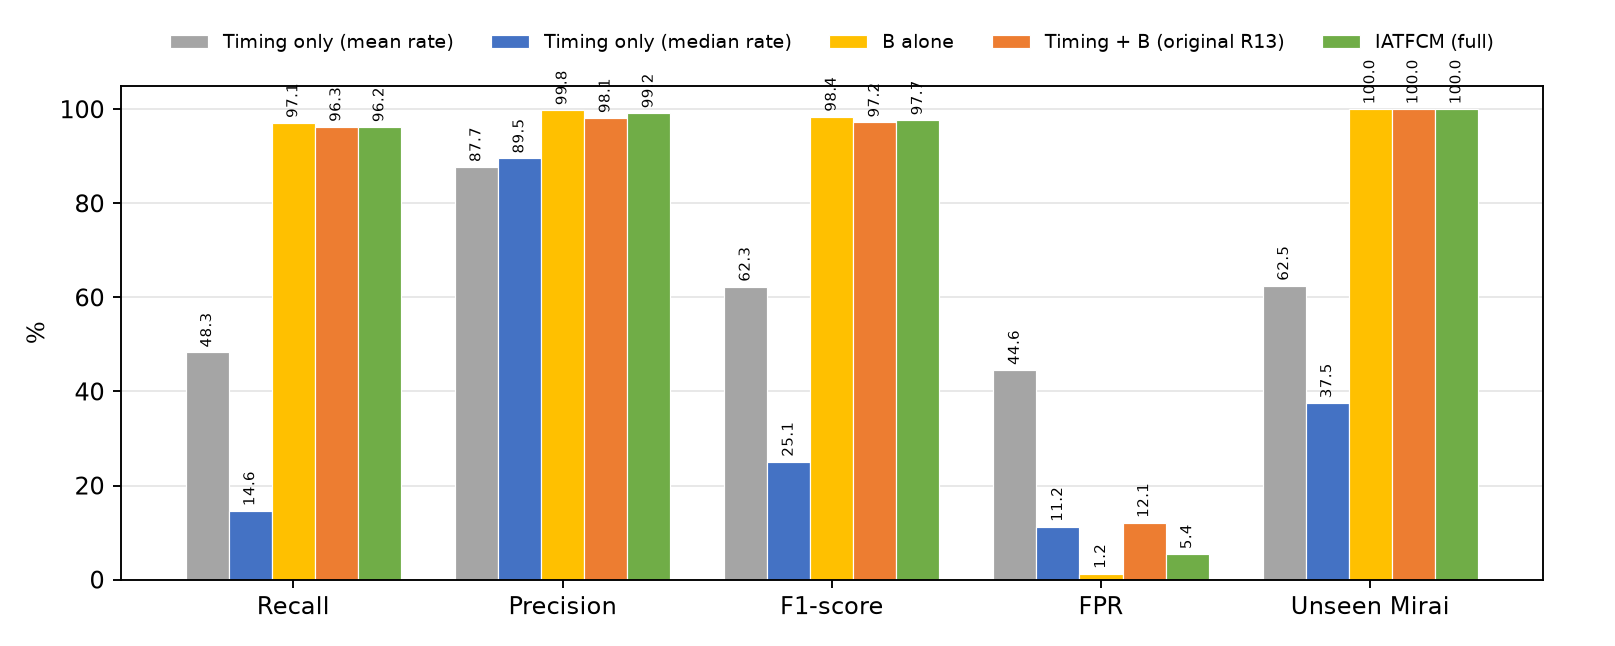
\includegraphics[width=\textwidth]{fig_abl_module1.png}
\caption{Ablation of Module 1: recall, precision, F1-score, false-positive rate and detection of the unseen Mirai windows for five versions of the detector.}
\label{fig:abl-m1}
\end{figure}

\textbf{Window size.} The window size $W$ was varied on windows that contain only the attack class, 15 windows per class and size. The F1-score of Module 1 was 99.39\% at $W = 10$ and 100\% at $W = 20$, 50 and 100. A window of 10 records holds too few IAT values for a stable CV, whereas windows larger than 20 do not improve the result and need more records before a decision, so they react later and mix more normal traffic into the window when an attack starts or ends. $W = 20$ is therefore used.

\subsection{Voting, zero-day check and quantization in Module 2}
\textbf{Voting rule.} Fig.~\ref{fig:abl-m2}(a) compares a plain majority vote over the 20 records with the attack-vote rule of IATFCM. With half of the window being benign background, the plain vote labels many attack windows as benign and classifies only 50.8\% of them correctly; the attack-vote rule keeps 96.3\% correct at that share. Over all known windows the window accuracy rises from 86.94\% to 98.47\%.

\textbf{Zero-day check.} Fig.~\ref{fig:abl-m2}(b) compares three ways of handling the unseen Mirai windows. Without a check, every Mirai window receives a known label. Rejecting windows whose mean maximum softmax probability\cite{hendrycks2017baseline} is below the 10th percentile of correctly classified known windows flags 58.3\% of the Mirai windows, at the cost of wrongly rejecting 10.5\% of the known attack windows. The nearest-neighbour distance of IATFCM flags all of the Mirai windows and wrongly rejects only 4.1\% of the known ones.

\textbf{Quantization.} At record level on 32,687 test records, the FP32 network reached 77.95\% accuracy and the INT8 network 77.85\%, with 98.51\% identical predictions, while the model size fell from 63.6~KB to 16.2~KB (74.6\% smaller). Quantization therefore costs 0.1 points of accuracy.

\begin{figure}[htbp]
\centering
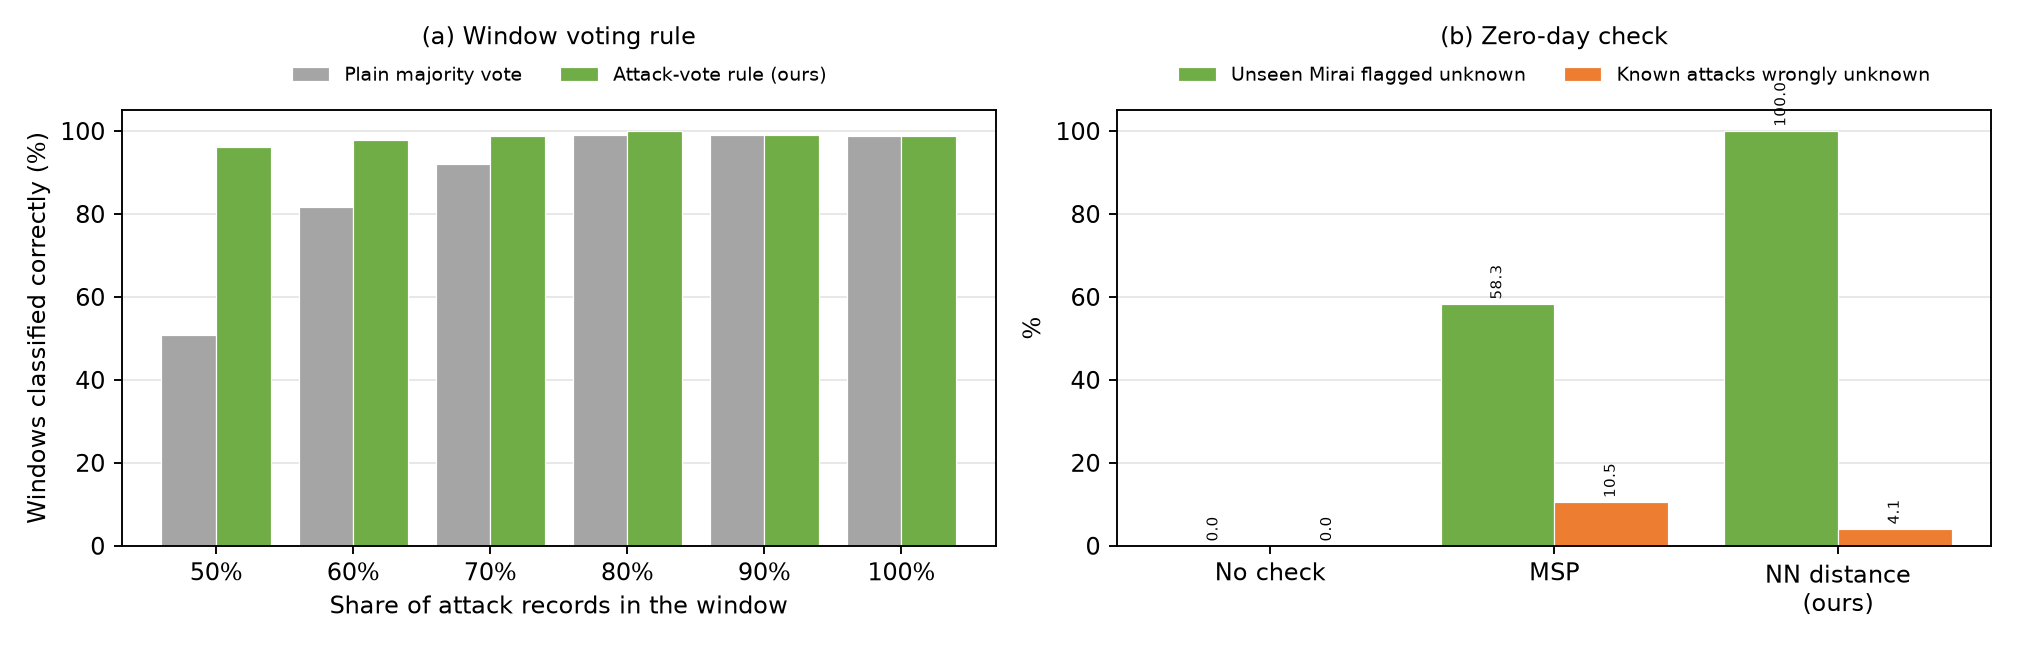
\includegraphics[width=\textwidth]{fig_abl_module2.png}
\caption{Ablation of Module 2: (a) window accuracy of the plain majority vote and the attack-vote rule against the share of attack records; (b) unseen Mirai windows flagged as unknown and known attack windows wrongly flagged, for no check, the maximum softmax probability (MSP) and the nearest-neighbour distance.}
\label{fig:abl-m2}
\end{figure}

\subsection{Escalation, verification and collateral damage in Module 3}
Module 3 was ablated on 164 attack windows (5 per attack class, 80\% attack share) that reached it. With the full ladder and verification, 99.39\% of the attacks were resolved, using 1.11 actions on average. Using only the first action resolves 89.63\%, so the escalation step recovers almost one attack in ten. Without the verification step, the first action would be assumed to work, and 10.37\% of the attacks would remain active without anyone noticing. Fig.~\ref{fig:abl-m3} also shows the collateral damage. Because IATFCM filters only the records that Module 2 marked as attacks, it dropped 14.59\% of the legitimate records in the attacked windows (benign records that were misclassified as attacks), against 100\% for the simple response of dropping every flagged window. For the 26 unseen-attack windows in this sample, the shape-based ladders and a single generic ladder resolved the same share (96.15\%); the shape routing did not increase the success rate here, but it reports the kind of attack to the analyst and chose a blocking action slightly more often (26.9\% against 23.1\% of the windows).

\begin{figure}[htbp]
\centering
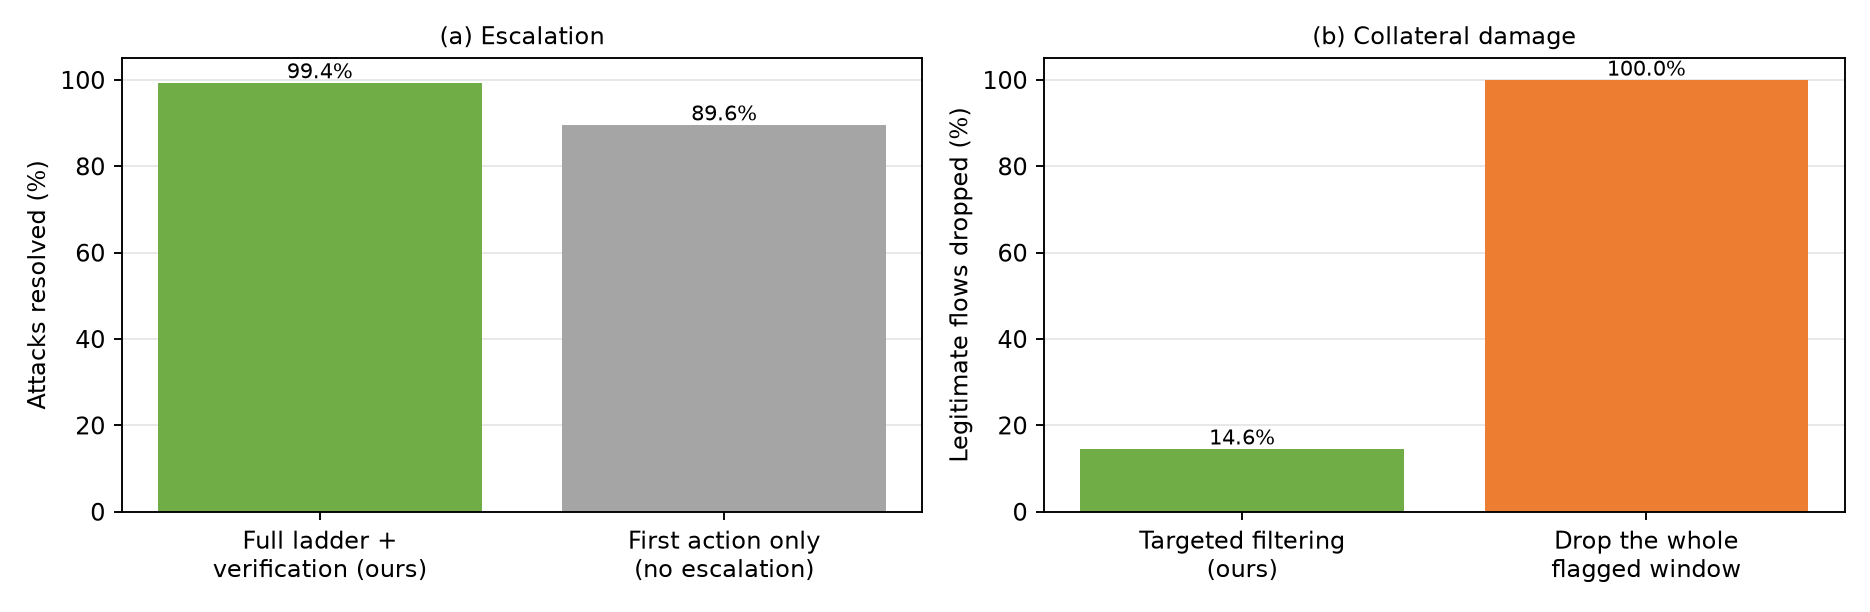
\includegraphics[width=0.95\textwidth]{fig_abl_module3.png}
\caption{Ablation of Module 3: (a) attacks resolved with the full escalation ladder and with the first action only; (b) legitimate records dropped by targeted filtering and by dropping the whole flagged window.}
\label{fig:abl-m3}
\end{figure}

\subsection{Gating by Module 1}
The last ablation removes the gate and runs Module 2 on every window of an end-to-end stream of 390 windows (normal, DDoS-SYN, Recon-PortScan, Mirai-udpplain and DoS-UDP phases, 10 random seeds). The results are given in Table~\ref{tab:abl-gate}. With the gate, Module 2 was called for 166 windows instead of 390, the computation per window fell from 13.22~ms to 8.53~ms (35.5\% less), and the number of benign windows that received a mitigation plan fell from 32 to 3, because Module 1 filters out most of the false alarms that the classifier alone would raise.

\begin{table}[htbp]
\tbl{Effect of the Module 1 gate on an end-to-end stream of 390 windows (230 benign).}
{\small
\begin{tabular}{lccc}
\toprule
Configuration & Module 2 calls & Time per window (ms) & Benign windows given a plan \\
\midrule
Module 2 on every window & 390 (100\%) & 13.22 & 32 \\
\textbf{IATFCM} (Module 1 gate) & 166 (42.6\%) & 8.53 & 3 \\
\bottomrule
\end{tabular}}
\label{tab:abl-gate}
\end{table}


% =====================================================================================
\section{Results and Discussion}\label{sec:results}
% =====================================================================================
This section compares IATFCM with the existing algorithms of Section~\ref{sec:lit} in terms of detection, recognition of unseen attacks, multiclass classification, computational cost and mitigation, and finally places it next to the results that the existing works report themselves.

\subsection{Experimental setup}
IATFCM and the compared algorithms are implemented in Python 3.14 with NumPy, pandas, scikit-learn and XGBoost and run on a desktop CPU. All supervised models are trained on 4,400 windows built from the training file (120 windows for each of the 30 known attack classes with an attack share drawn between 50\% and 100\%, and 800 benign windows), and all algorithms are tested on the same 1,824 test windows described in Section~\ref{sec:ablation}. The Mirai family is excluded from every training set. To compare under one protocol, the core technique of each existing work was re-implemented from its description (Table~\ref{tab:compared}); these are re-implementations, not the authors' code, and settings that the papers do not report were chosen as reasonable defaults. BCT and DNN-BiLSTMQ require deep learning toolkits that were not used here, so they are compared through the CICIoT2023 results their authors report (Section~\ref{sec:published}).

\begin{table}[htbp]
\tbl{Existing algorithms re-implemented for the comparison.}
{\small
\begin{tabular}{p{1.7cm}p{8.9cm}p{2.1cm}}
\toprule
Short name & Re-implemented core technique & Compared in \\
\midrule
DT-3$\sigma$\cite{dynamic_ids2025} & Mean packets/s and bytes/s of the window; alarm when either exceeds the mean plus three standard deviations of benign training windows (label-free) & Detection \\
SAE-PSVM\cite{nie2025intrusion} & Stacked autoencoder (46--32--16 code) on log-scaled records, RBF-SVM with $C$ and $\gamma$ tuned by particle swarm optimisation (8 particles, 6 iterations); attack window if at least half of its records are attacks & Detection \\
PP-TTF\cite{ertam2026privacy} & 30 IAT-only descriptors: mean, standard deviation, minimum, maximum, range, entropy and CV of the IAT over the last 3, 5, 10 and 20 records, mean log IAT and burst share; Random Forest with 100 trees, depth 10, balanced classes & Detection and classification \\
HFF-XGB\cite{solpan2026hybrid} & Mean, standard deviation, minimum, maximum and median of all 46 features over the window (230 attributes); XGBoost with 200 trees of depth 6 & Classification \\
DNN-KDQ\cite{umar2025energy} & 46--64--32--31 student network distilled from the soft labels of the Random Forest teacher, quantized to INT8, with the same window vote as IATFCM & Classification \\
\bottomrule
\end{tabular}}
\label{tab:compared}
\end{table}

\subsection{Detection performance}
Fig.~\ref{fig:cmp-share} compares the share of attack windows detected by DT-3$\sigma$, SAE-PSVM, PP-TTF and IATFCM as the share of attack records in the window grows from 50\% to 100\%, much as the payload size is varied in other performance studies. All methods detect more attacks as the attack becomes a larger part of the window. IATFCM detects 85.6\% of the windows that are only half attack and 99.2--100\% of the windows with at least 80\% attack records. The label-free DT-3$\sigma$ detects at most 11.0\% at any share: CICIoT2023 packet rates are heavy-tailed, so the mean plus three standard deviations of benign traffic lies far above most attack windows. SAE-PSVM rises from 68.9\% to 94.7\%, while PP-TTF detects 94.7--100\% at every share and is the strongest detector when only half of the window is attack.

\begin{figure}[htbp]
\centering
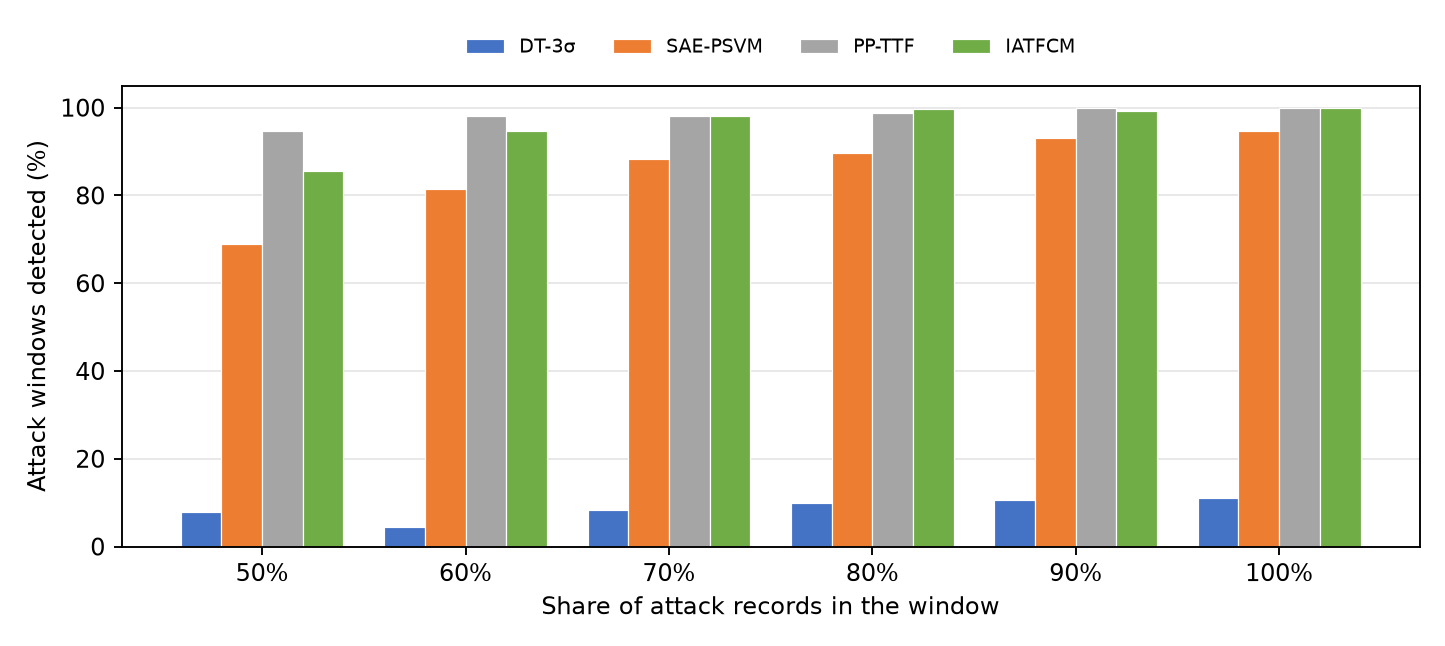
\includegraphics[width=\textwidth]{fig_cmp_detection_by_share.png}
\caption{Attack windows detected by DT-3$\sigma$, SAE-PSVM, PP-TTF and IATFCM for attack shares of 50--100\% of the window.}
\label{fig:cmp-share}
\end{figure}

The overall detection metrics are compared in Fig.~\ref{fig:cmp-detmetrics}. IATFCM reaches a recall of 96.21\%, a precision of 99.15\%, an F1-score of 97.66\% and a false-positive rate of 5.42\%. Compared with the only other label-free method, DT-3$\sigma$ (F1-score 15.97\%), the F1-score is 81.7 points higher, and compared with SAE-PSVM (92.50\%) it is 5.2 points higher. The supervised PP-TTF detector is better on these known attack types, with an F1-score of 99.11\% and a false-positive rate of 0.42\%. This is expected, because PP-TTF is trained with labelled attack windows of the same attack types and attack shares as the test windows, whereas Module 1 of IATFCM has seen only benign traffic and has to be retrained for nothing when a new attack type appears. The strength of PP-TTF also confirms the premise of this work, that the inter-arrival time carries a strong signal for IoT attacks in CICIoT2023.

\begin{figure}[htbp]
\centering
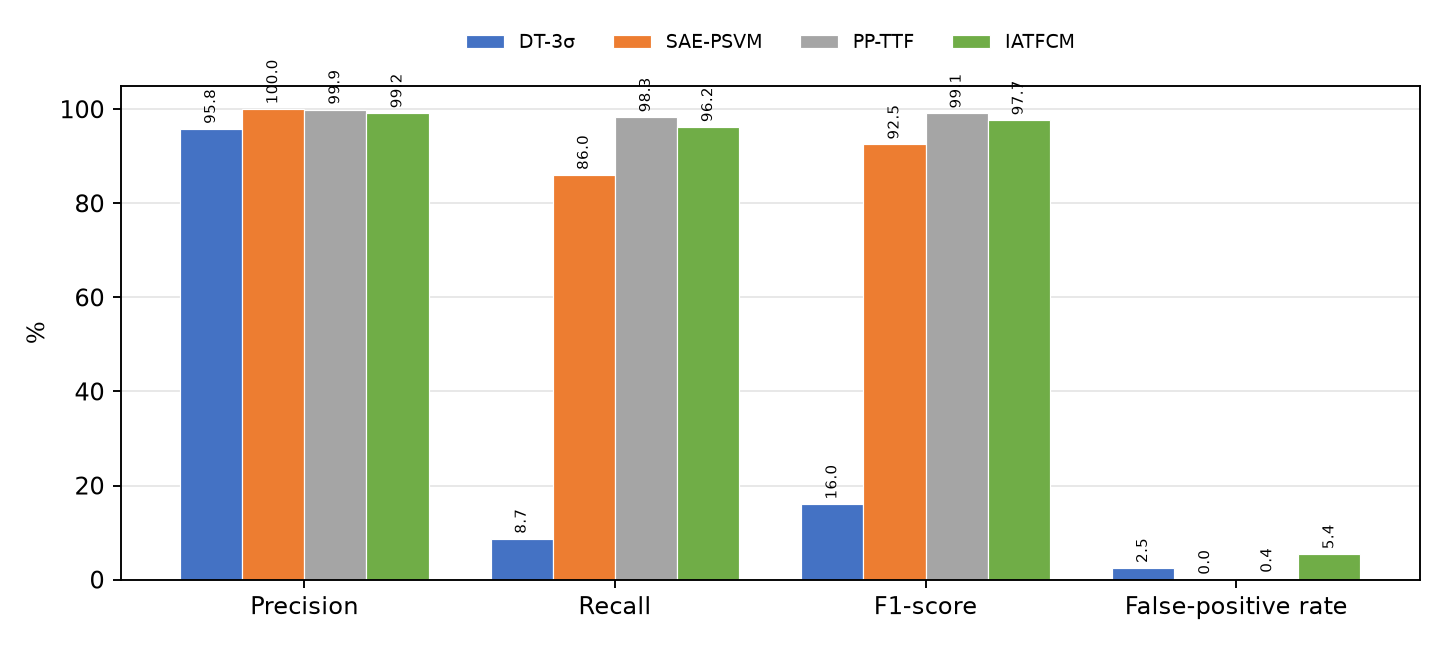
\includegraphics[width=\textwidth]{fig_cmp_detection_metrics.png}
\caption{Precision, recall, F1-score and false-positive rate of the detection stage of each algorithm.}
\label{fig:cmp-detmetrics}
\end{figure}

Fig.~\ref{fig:cmp-family} breaks the detection rate down by attack family. All methods except DT-3$\sigma$ detect nearly every DDoS and DoS window. The differences appear for the attacks that do not flood the network. IATFCM detects 88.3\% of the reconnaissance, 90.6\% of the spoofing, 94.4\% of the web and 87.5\% of the brute-force windows, where SAE-PSVM detects only 67.5\%, 35.4\%, 80.2\% and 56.2\%. PP-TTF is higher on these families (93.8--100\%), again with the advantage of supervised training on them.

\begin{figure}[htbp]
\centering
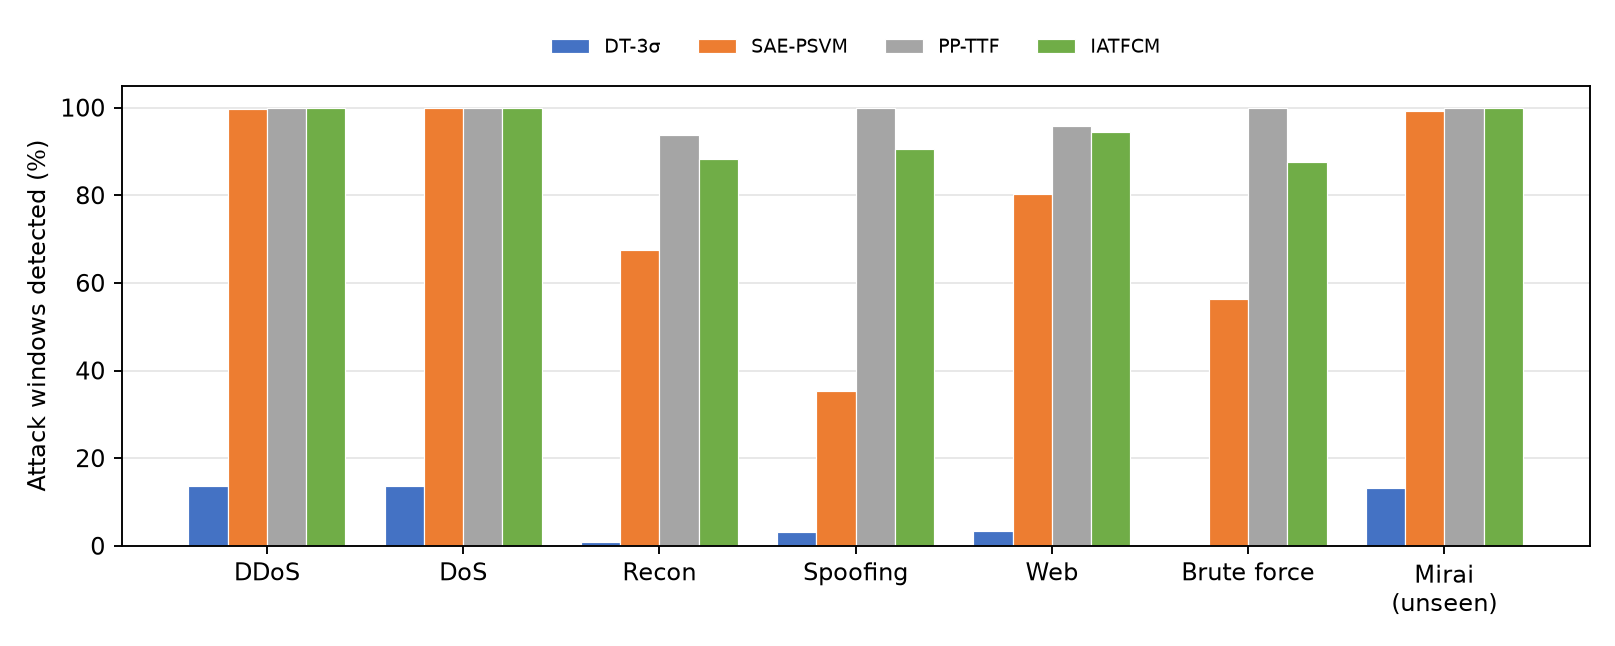
\includegraphics[width=\textwidth]{fig_cmp_detection_family.png}
\caption{Attack windows detected for each attack family, including the unseen Mirai family.}
\label{fig:cmp-family}
\end{figure}

\subsection{Detection and recognition of unseen attacks}
For the 144 windows of the held-out Mirai family, two different questions matter: is the window flagged, and is it recognised as something new? IATFCM, PP-TTF and SAE-PSVM flagged 100\%, 100\% and 99.3\% of the Mirai windows as attacks, and DT-3$\sigma$ only 13.2\%. The supervised binary detectors catch Mirai because these floods resemble the known floods they were trained on. The difference appears at the classification stage (Fig.~\ref{fig:cmp-clsmetrics}): HFF-XGB assigned 141 of the 144 Mirai windows to DDoS-UDP\_Fragmentation, PP-TTF spread them over DDoS-SlowLoris, DDoS-HTTP\_Flood and DoS-TCP\_Flood, and DNN-KDQ over DDoS-ACK\_Fragmentation and DDoS-UDP\_Flood, so none of them recognised a single Mirai window as unknown. IATFCM labelled all 144 as possible zero-day attacks, with a median zero-day score of 3.69 against 0.52 for known attack windows (Fig.~\ref{fig:zeroday}). This matters for the response: a wrong known label selects the policy of another attack, whereas the unknown label sends the window to the shape-based containment of Module 3.

\begin{figure}[htbp]
\centering
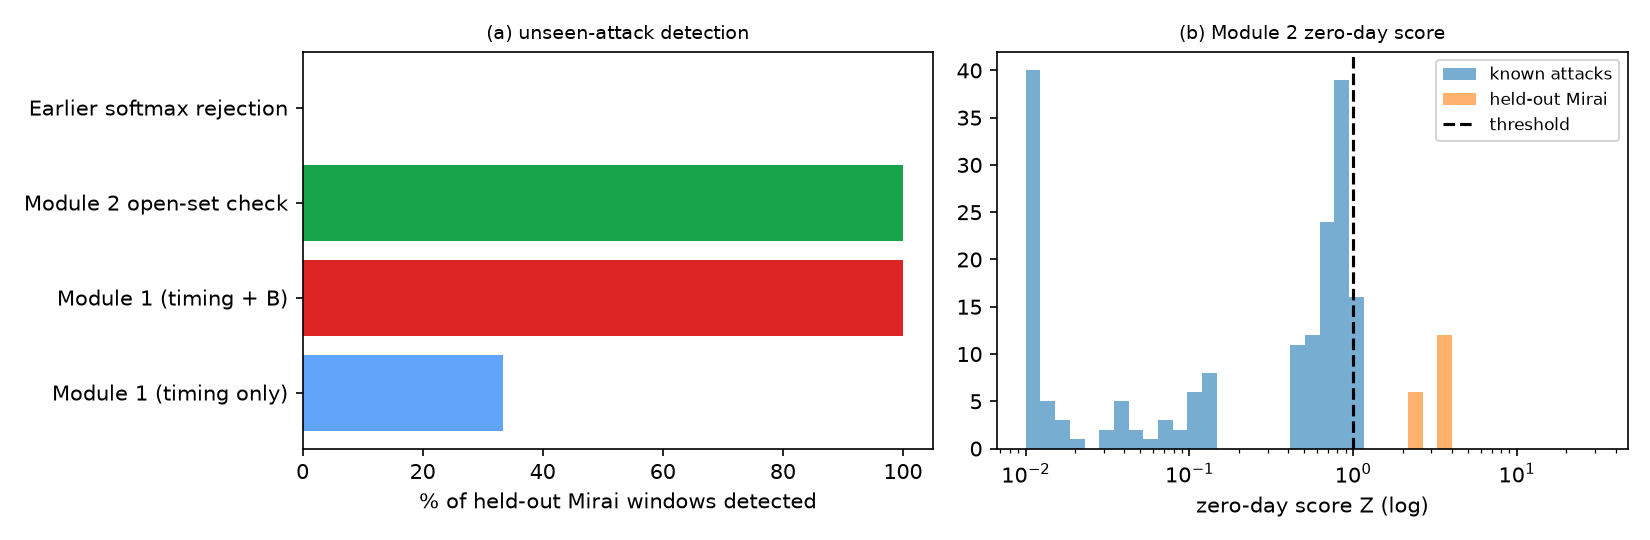
\includegraphics[width=\textwidth]{fig_zero_day_analysis.png}
\caption{Unseen Mirai analysis: (a) Mirai windows detected by the timing-only detector, by the full Module 1 and by the zero-day check of Module 2, and by the confidence-based rejection used in our earlier work; (b) distribution of the zero-day score $Z_t$ for known attack windows and Mirai windows, with the threshold at 1.}
\label{fig:zeroday}
\end{figure}

\subsection{Multiclass classification performance}
Fig.~\ref{fig:cmp-clsshare} shows the share of windows of the 31 known classes that each classifier labels correctly as the attack share changes, and Fig.~\ref{fig:cmp-clsmetrics} summarises accuracy, macro-F1, family accuracy and the recognition of unseen attacks. The Random Forest of IATFCM classified 92.98\% of the windows correctly (macro-F1 94.54\%, family accuracy 94.05\%) and stays between 92.9\% and 97.1\% at every share, because its attack-vote rule ignores the benign background. HFF-XGB is the most accurate classifier on the known classes, with 98.45\% accuracy and 98.34\% macro-F1. It achieves this with 230 attributes per window and, as shown above, without any means of recognising an unseen attack. PP-TTF reaches 90.06\% but drops to 74.2\% when half of the window is benign, since it has only the timing of the window to go on. Among the compact edge models, the INT8 network of IATFCM is more accurate than the re-implemented DNN-KDQ (68.51\% against 65.06\%; macro-F1 67.57\% against 60.83\%), at 16.2~KB against 6.2~KB.

\begin{figure}[htbp]
\centering
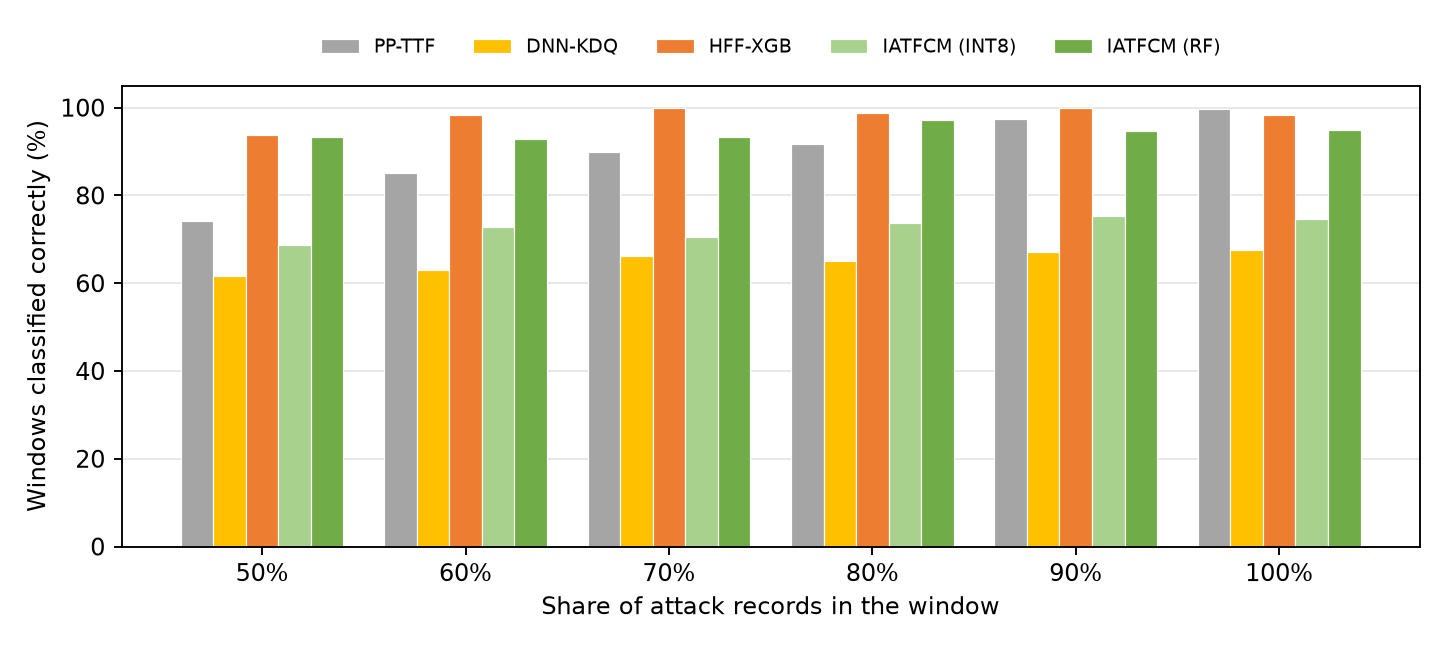
\includegraphics[width=\textwidth]{fig_cmp_classification_by_share.png}
\caption{Windows of the known classes classified correctly by PP-TTF, DNN-KDQ, HFF-XGB and the INT8 and Random Forest classifiers of IATFCM, for attack shares of 50--100\%.}
\label{fig:cmp-clsshare}
\end{figure}

\begin{figure}[htbp]
\centering
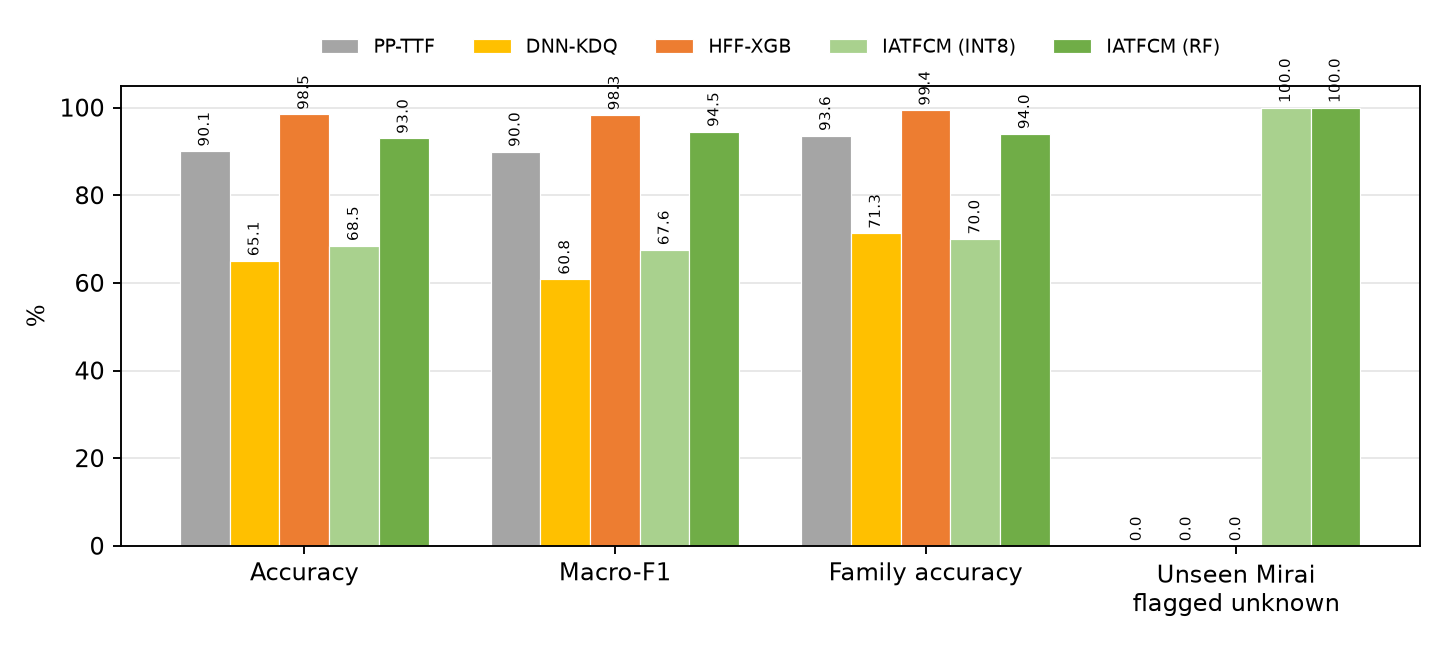
\includegraphics[width=\textwidth]{fig_cmp_classification_metrics.png}
\caption{Accuracy, macro-F1 and family accuracy on the known classes, and the share of unseen Mirai windows recognised as unknown.}
\label{fig:cmp-clsmetrics}
\end{figure}

At record level, on the 32,687 test records of the known classes, the Random Forest reached 90.85\% accuracy, 79.34\% macro-F1 and 93.42\% family accuracy. All flood classes reach an F1-score of at least 0.97 (Fig.~\ref{fig:m2perclass}); the weaker classes are the rare web and reconnaissance attacks, such as SQL injection (0.37), XSS (0.46), uploading attack (0.32) and Recon-PingSweep (0.29), whose errors mostly stay inside the correct family (Fig.~\ref{fig:m2family}).

\begin{figure}[htbp]
\centering
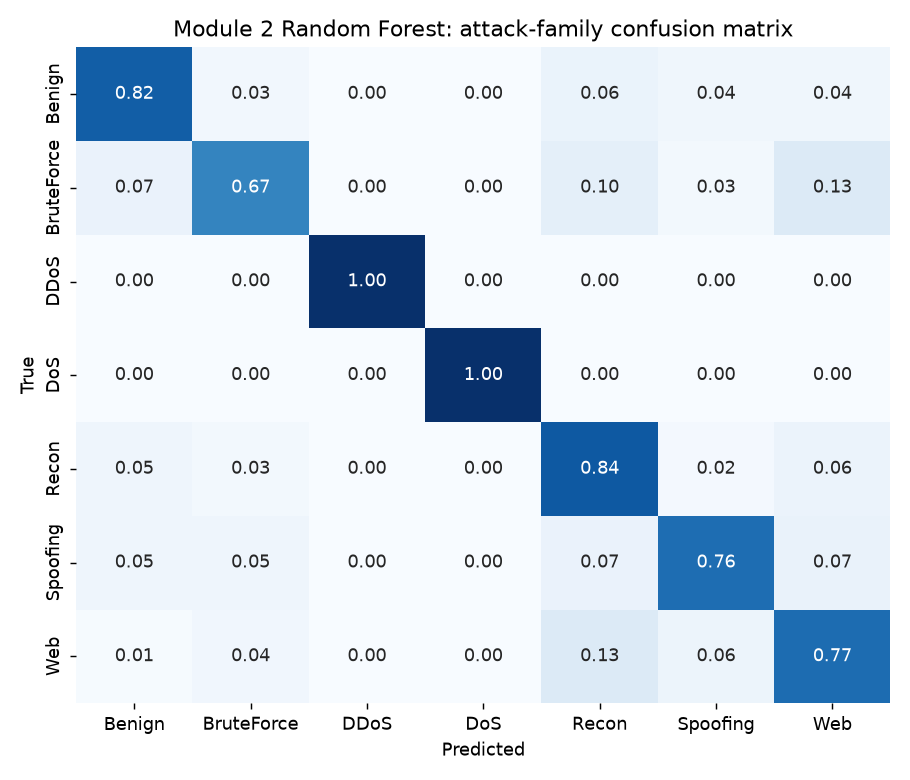
\includegraphics[width=0.62\textwidth]{m2_family_confusion.png}
\caption{Normalised attack-family confusion matrix of the Random Forest of IATFCM on the test records.}
\label{fig:m2family}
\end{figure}

\begin{figure}[htbp]
\centering
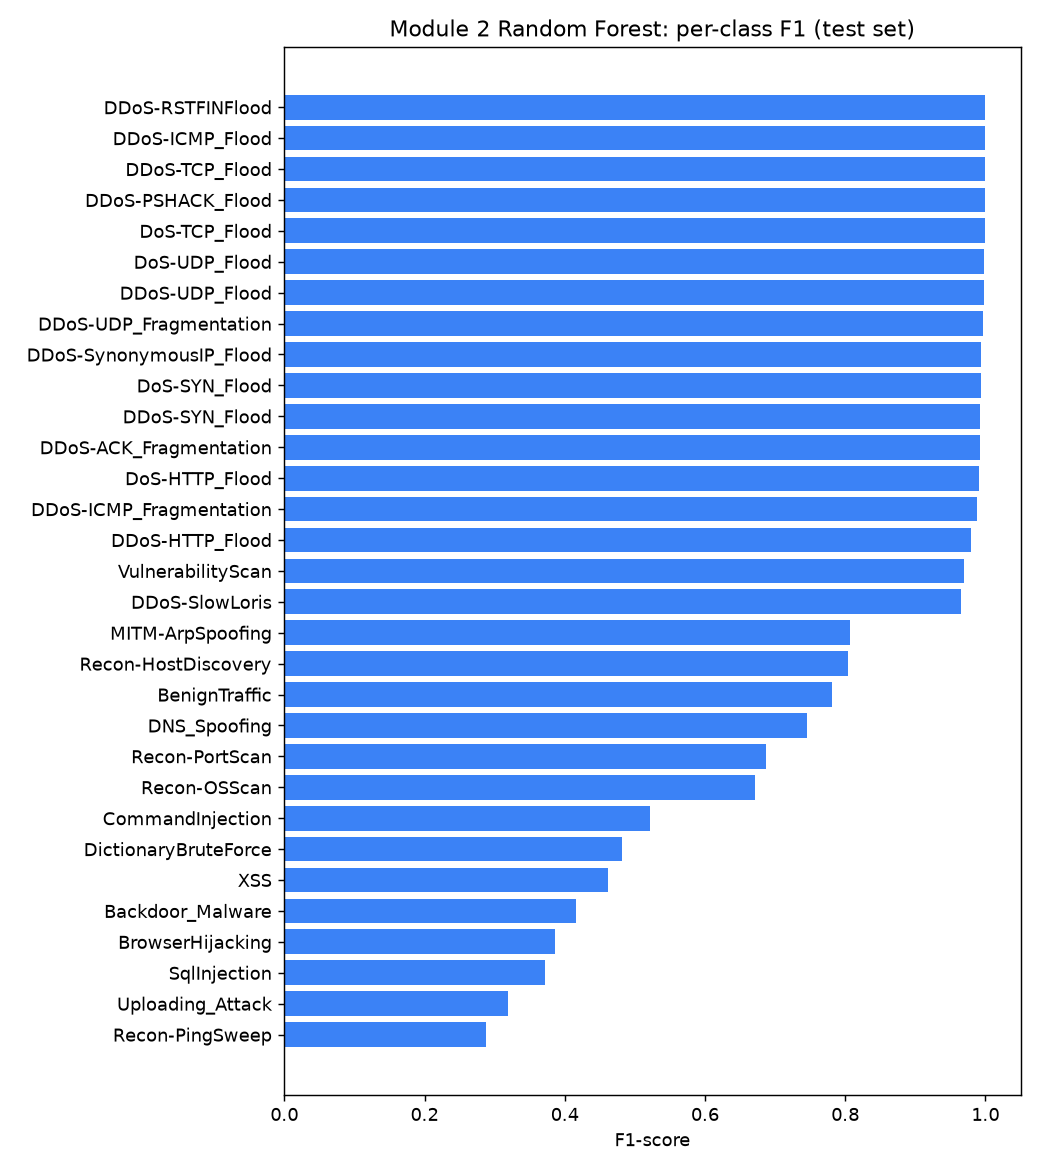
\includegraphics[width=0.68\textwidth]{m2_per_class_f1.png}
\caption{Per-class F1-score of the Random Forest of IATFCM on the test records.}
\label{fig:m2perclass}
\end{figure}

\subsection{Computational cost}
Fig.~\ref{fig:cmp-cost} and Table~\ref{tab:cost} compare the latency per window and the model size. On the detection side, Module 1 needs 2.68~ms per window, close to SAE-PSVM (2.83~ms) and less than half of PP-TTF (5.85~ms); most of its time is spent on the nearest-neighbour search of the behaviour deviation, and its 1.6~MB size is the benign reference set of that search. DT-3$\sigma$ is the cheapest method but, as shown above, detects few attacks. On the classification side, the Random Forest of IATFCM is accurate but large (115~MB) and the slowest model (11.37~ms per window, including the zero-day search), so it suits a gateway rather than a constrained device. For such devices, the INT8 network needs only 16.2~KB, and its inference takes 0.52~ms per window; the complete Module 2 call takes 5.83~ms because the zero-day search dominates. Since Module 2 runs only on the windows that Module 1 forwards (42.6\% in the end-to-end stream), the average cost per window of the whole pipeline is 8.53~ms (Table~\ref{tab:abl-gate}).

\begin{figure}[htbp]
\centering
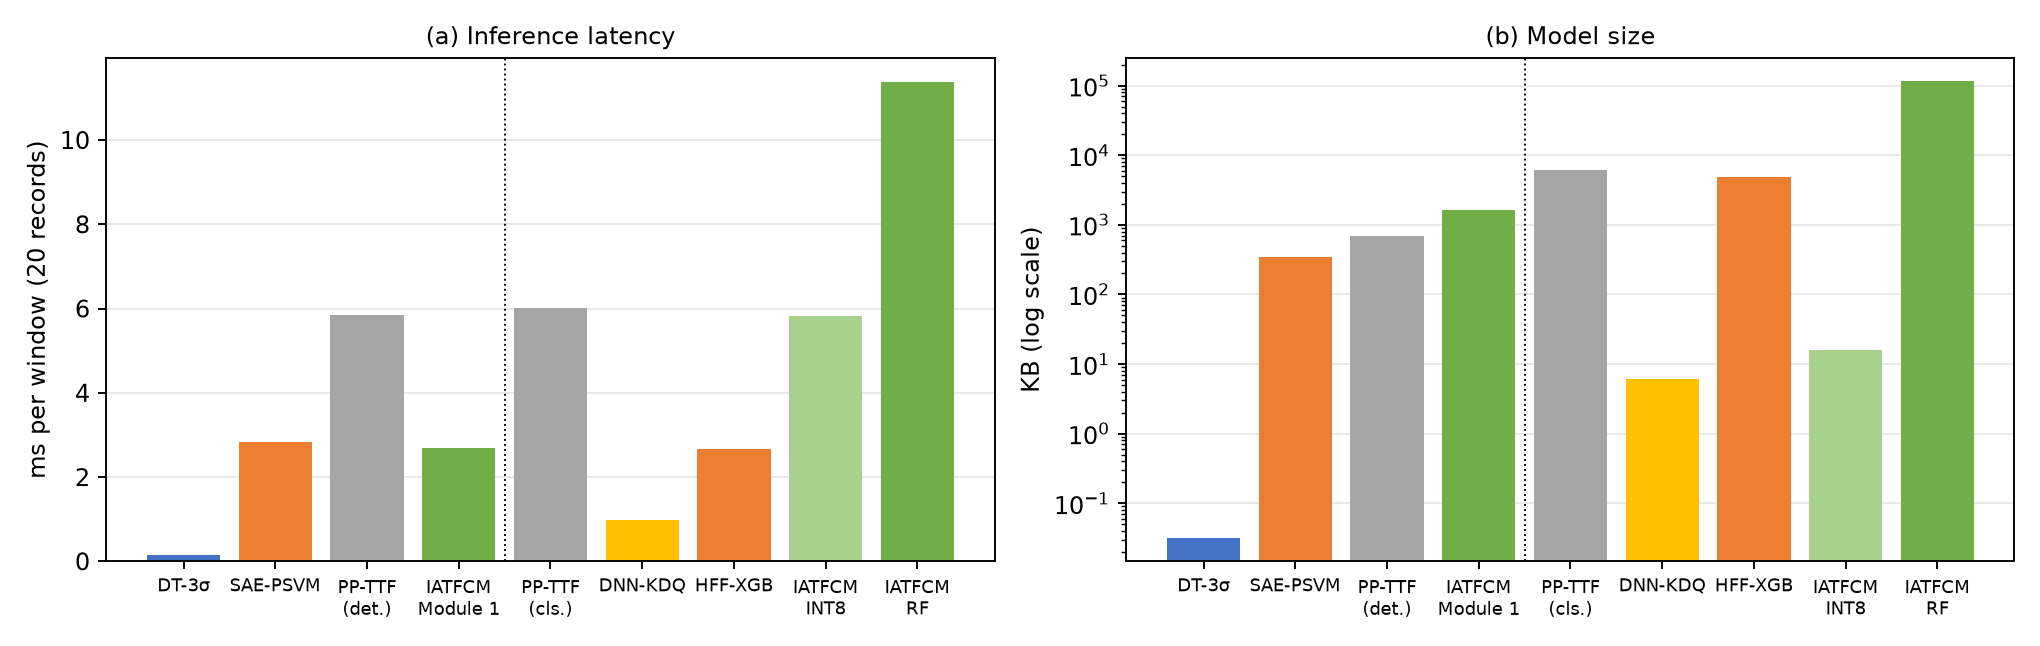
\includegraphics[width=\textwidth]{fig_cmp_cost.png}
\caption{(a) Inference latency per window of 20 records and (b) model size of each algorithm; detection methods are left of the dotted line, classifiers right of it.}
\label{fig:cmp-cost}
\end{figure}

\begin{table}[htbp]
\tbl{Features, model size and latency of the compared algorithms.}
{\small
\begin{tabular}{llccc}
\toprule
Algorithm & Stage & Features & Size (KB) & Latency (ms/window) \\
\midrule
DT-3$\sigma$ & Detection & 2 & 0.03 & 0.16 \\
SAE-PSVM & Detection & 46 & 340.2 & 2.83 \\
PP-TTF & Detection & 30 & 683.1 & 5.85 \\
\textbf{IATFCM} Module 1 & Detection & 4 (from 46) & 1,619.6 & 2.68 \\
\midrule
PP-TTF & Classification & 30 & 6,225.1 & 6.00 \\
HFF-XGB & Classification & 230 & 4,906.1 & 2.67 \\
DNN-KDQ & Classification & 46 & 6.2 & 0.97 \\
\textbf{IATFCM} INT8 & Classification & 46 & 16.2 & 5.83 \\
\textbf{IATFCM} Random Forest & Classification & 46 & 115,555.0 & 11.37 \\
\bottomrule
\end{tabular}}
\label{tab:cost}
\end{table}

\subsection{Mitigation performance}
None of the compared algorithms applies a response, so the mitigation stage of IATFCM is evaluated on its own, through the full pipeline and driven by the predictions of Module 2, on 645 windows: 15 windows for each of the 33 attack classes (80\% attack records) and 150 benign windows. 489 windows reached Module 3, 86.5\% of them through a class policy and 13.5\% through the zero-day route. Known attacks were routed to the policy family of their true class in 94.82\% of the cases, and 96.11\% of the plans were verified by Module 1 to bring the risk below 0.35. The mean risk fell from 0.73 to 0.18 and the mean CV after mitigation was 0.99, close to the normal value of 1.0. 85.5\% of the plans needed a single action, the first action removed 82.24\% of the targeted packet rate, and 62.4\% of the plans could start automatically. Table~\ref{tab:m3family} and Fig.~\ref{fig:m3family} give the results per policy family. The filtering families start automatically and are resolved in 95.6--98.3\% of the windows, whereas the reconnaissance, spoofing, web, credential and malware plans wait for an analyst because their first action blocks traffic or the classifier is less confident on these classes. All 45 unseen Mirai windows took the zero-day route; 37 of them (82.2\%) were recognised as constant-rate floods from their traffic shape, and 95.56\% were resolved. No benign window of this evaluation reached Module 3.

\begin{table}[htbp]
\tbl{Mitigation results per policy family (645-window evaluation driven by Module 2 predictions).}
{\small
\begin{tabular}{lccccc}
\toprule
Policy family & Windows & Resolved & Automatic & Single action & Volume removed \\
\midrule
Volumetric flood        & 90 & 96.7\%  & 100\% & 76.7\%  & 74.1\% \\
TCP state exhaustion    & 60 & 98.3\%  & 100\% & 76.7\%  & 79.5\% \\
Fragmentation           & 45 & 95.6\%  & 100\% & 84.4\%  & 76.0\% \\
Slow application        & 45 & 97.8\%  & 100\% & 93.3\%  & 83.1\% \\
Reconnaissance          & 60 & 93.3\%  & 0\%   & 93.3\%  & 95.4\% \\
Spoofing / MITM         & 30 & 100\%   & 0\%   & 100\%   & 98.6\% \\
Web application         & 66 & 90.9\%  & 0\%   & 84.9\%  & 85.7\% \\
Credential              & 12 & 100\%   & 0\%   & 100\%   & 84.6\% \\
Malware / backdoor      & 15 & 100\%   & 0\%   & 100\%   & 100\% \\
Zero-day (traffic shape)& 66 & 97.0\%  & 98.5\% & 81.8\% & 72.1\% \\
\midrule
All                     & 489 & 96.1\% & 62.4\% & 85.5\% & 82.2\% \\
\bottomrule
\end{tabular}}
\label{tab:m3family}
\end{table}

\begin{figure}[htbp]
\centering
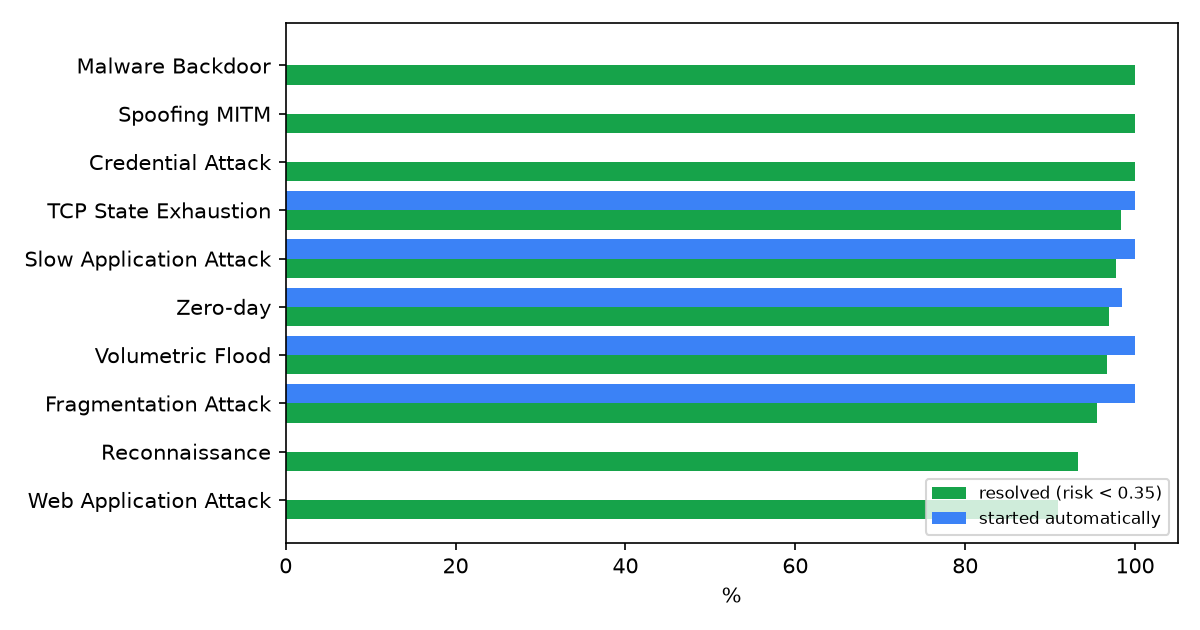
\includegraphics[width=0.8\textwidth]{fig_mitigation_by_family.png}
\caption{Share of windows resolved after mitigation (risk below 0.35) and share of plans started automatically, for each policy family.}
\label{fig:m3family}
\end{figure}

In the end-to-end stream of 390 windows, Module 1 detected 158 of the 160 attack windows (98.75\%) and raised 8 false alarms on the 230 normal windows (3.48\%), and 57.4\% of the windows bypassed Modules 2 and 3 (Fig.~\ref{fig:routing}). Module 3 executed 161 plans, 74.5\% through a class policy and 25.5\% through the zero-day route, and verified 98.76\% of them: 136 with the first action and 23 after one escalation. Three benign windows received a plan; their ladders include blocking, so in deployment they would wait for an analyst instead of disconnecting a device.

\begin{figure}[htbp]
\centering
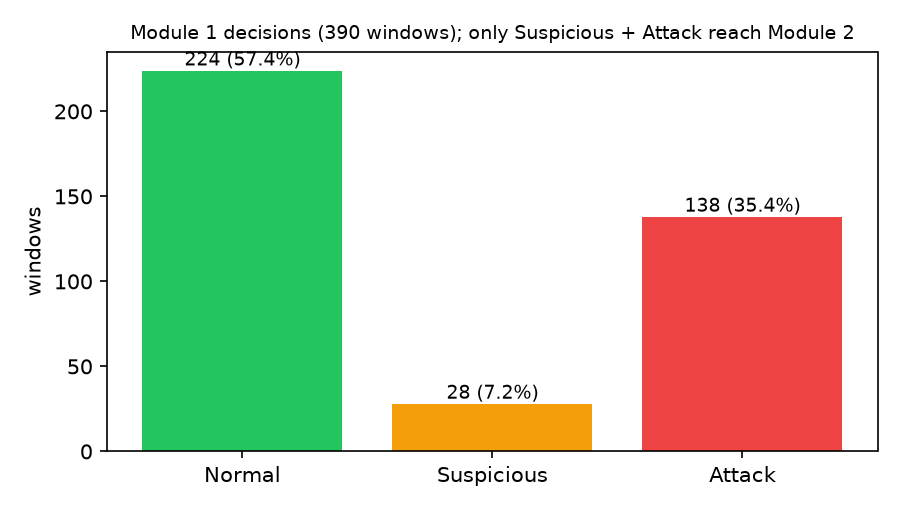
\includegraphics[width=0.72\textwidth]{fig_module2_invocation.png}
\caption{Module 1 decisions for the 390 windows of the end-to-end stream; only suspicious and attack windows reach Module 2.}
\label{fig:routing}
\end{figure}

\subsection{Comparison with published results}\label{sec:published}
Table~\ref{tab:published} lists the results that the existing works report in their own papers. These numbers come from different datasets, class sets and splits, so they indicate the operating range of each method rather than a direct ranking. Two works report on CICIoT2023. BCT reports a macro-F1 of 0.4747 with a 0.10~MB model, and DNN-BiLSTMQ an accuracy of 93.95\% with a 31.3~KB model. The record-level Random Forest of IATFCM reaches a macro-F1 of 0.7934 and an accuracy of 90.85\% on the 31 known classes, and its INT8 network 77.85\% with 16.2~KB. Unlike all listed works, IATFCM also recognises unseen attacks as unknown and verifies a response to every detected attack.

\begin{table}[htbp]
\tbl{Results reported by the existing works (from their papers) and by IATFCM.}
{\small
\begin{tabular}{llll}
\toprule
Algorithm & Dataset & Reported result & Size / latency \\
\midrule
PP-TTF\cite{ertam2026privacy} & Robotic Wi-Fi, 5 classes & Binary F1 0.906; multiclass accuracy 0.782 & -- \\
HFF-XGB\cite{solpan2026hybrid} & AWID3, 14 classes & Accuracy and F1 above 0.98 & -- \\
SAE-PSVM\cite{nie2025intrusion} & Wireless node traffic & False detection rate below 6\% & -- \\
BCT\cite{tuman2025edge} & CICIoT2023 & Macro-F1 0.4747 & 0.10 MB / 0.1131 ms per sample \\
DNN-BiLSTMQ\cite{misrak2025lightweight} & CICIoT2023 & Accuracy 93.95\% & 31.3 KB \\
DT-3$\sigma$\cite{dynamic_ids2025} & CICIDS2017, NSL-KDD & Accuracy 94.7--96.2\% & 5.1\% CPU \\
DNN-KDQ\cite{umar2025energy} & CICIDS2017 & Accuracy 99.43\% & 20.18 KB / 0.07 ms per sample \\
\midrule
\textbf{IATFCM} (Random Forest) & CICIoT2023, 31 known classes & Accuracy 90.85\%; macro-F1 0.7934 & 115.6 MB \\
\textbf{IATFCM} (INT8) & CICIoT2023, 31 known classes & Accuracy 77.85\%; macro-F1 0.6317 & 16.2 KB \\
\bottomrule
\end{tabular}}
\label{tab:published}
\end{table}

\subsection{Discussion and limitations}
The comparison shows where IATFCM stands. It is the most accurate of the label-free detectors and the only algorithm that recognises unseen attacks as unknown and acts on them, and its gate saves both computation and false responses. Supervised methods that are trained on the very attack types and attack shares of the test (PP-TTF for detection, HFF-XGB for classification) are more accurate on those known attacks, at the price of needing labelled attack data and, for HFF-XGB, 230 attributes per window. Several limitations remain. The CSV release of CICIoT2023 has no packet timestamps and its rows are shuffled, so the windows are assembled from test records rather than taken from a continuous capture. The network controller of Module 3 is simulated and the efficacy of each action is an assumption. The behaviour deviation alone detects as well as the full fuzzy system on this dataset. The rare web and reconnaissance classes have few records, and the Random Forest is large. Finally, latency was measured on a desktop CPU rather than on IoT hardware.


% =====================================================================================
\section{Conclusion}\label{sec:conclusion}
% =====================================================================================
This paper proposed IATFCM, an algorithm that detects, classifies and mitigates attacks in resource-constrained IoT networks. A Mamdani fuzzy gate combines the inter-arrival time statistics of each window with a behaviour deviation learned only from benign traffic, a quantized classifier with an attack-vote rule and a nearest-neighbour check names known attacks and recognises unseen ones, and attack-specific policies with shape-based containment respond to every detected attack and verify the response with the same gate. On CICIoT2023 with the Mirai family held out, IATFCM detected 96.21\% of the attack windows with a 99.15\% precision, raised the F1-score of label-free detection from 15.97\% (DT-3$\sigma$) to 97.66\%, and recognised all unseen Mirai windows as unknown, which none of the compared classifiers did. The INT8 network needs 16.2~KB, 74.6\% less than its FP32 version. Module 3 routed 94.82\% of the known attacks to the correct policy and verified 96.11\% of the mitigations across 33 attack classes, while dropping 85.4\% less legitimate traffic than blocking the whole window, and the gate reduced the computation per window by 35.5\% and the benign windows given a mitigation plan from 32 to 3. Supervised competitors trained on the same attack types remain more accurate on known attacks, which IATFCM trades for label-free detection, recognition of unseen attacks and a verified response.

\section{Future Scope}
Future work will evaluate IATFCM on raw packet captures with real timestamps and continuous traffic, deploy the INT8 network and the mitigation actions on physical IoT gateways to measure latency and energy, learn the weights of the fuzzy rules from data so that the timing rules add fewer false alarms, replace the large Random Forest with a compact gradient-boosted model, and improve the classification of the rare web and reconnaissance attacks.

\section*{Disclosure statement}
The authors report there are no competing interests to declare.

\section*{Data availability statement}
The CICIoT2023 dataset used in this study is publicly available from the Canadian Institute for Cybersecurity. The implementation of IATFCM is available at \url{https://github.com/sahamon-141/Capstone-2}.

\bibliographystyle{tfp}
\bibliography{references}

\end{document}
